\chapter{Time-resolved brain dynamics during task performance} \label{chapter:ch5}
%Here you can see a citation: \cite{atc13}.

Dynamic approaches to analyse resting-state data have blossomed in recent years \citep{Chang2010,Preti2017}, but task-related paradigms to study cognition are yet to fully benefit from these methods. Most analyses available to date are based on sliding-window procedures \citep{Kucyi2014,Di2015,Gonzalez-Castillo2018}, thus relying on averaging over relatively long intervals of data. As a consequence, these methods do not fully explore the dynamic range that fMRI is able to unveil, which is down to sub-second scale. Point process analysis \citep{Tagliazucchi2012,Liu2013} select subsets of single fMRI frames when a seed is highly active and, when those are clustered, reoccurring patterns are unveiled containing all regions that co-activate with that region of interest. This allows brain function to be linked to specific moments of the experiment at frame resolution. 

With the above in mind, in this chapter I introduce a method to examine moment-to-moment changes in brain connectivity during performance of a task, which has been published in the peer-reviewed journal NeuroImage \citep{Freitas2020}. I illustrate that this analysis captures information on brain function which is impossible to obtain using conventional static approaches. Given its ability to concentrate the analysis on limited amounts of data, this represents a promising avenue for the study of the dynamic features of task-modulated brain function in clinical or young populations. Therefore, on a second study, I apply this method to a data set in which preterm-born young adolescents and age-matched controls perform a task which involves movie watching and emotion regulation. We thus argue that explicitly examining changes in connectivity patterns is paramount to advance our understanding of how different brain areas dynamically communicate when presented with a set of cues, and of what abnormalities may arise in this interplay as a consequence of clinical conditions such as preterm birth. 

\section{Journal Article: Time-resolved effective connectivity in task fMRI: psychophysiological interactions of co-activation patterns (PPI-CAPs)} \label{section:ppicaps_method}

\begin{center}
 \textit{(This article has been published in NeuroImage on Volume 212, 15 May 2020)}
 
Lorena G. A. Freitas\textsuperscript{a,b,e}, 
Thomas A. W. Bolton\textsuperscript{a,b},  
Benjamin E. Krikler\textsuperscript{c}, 
Delphine Jochaut\textsuperscript{d}, 
Anne-Lise Giraud\textsuperscript{d}, 
Petra S. Hüppi\textsuperscript{e},
Dimitri Van De Ville\textsuperscript{a,b} 

\end{center}
\textsuperscript{a} Institute of Bioengineering, École Polytechnique Fédérale de Lausanne, Switzerland \\
\textsuperscript{b} Department of Radiology and Medical Informatics, University of Geneva, Switzerland \\
\textsuperscript{c} Department of Physics, University of Bristol, United Kingdom \\ 
\textsuperscript{d} Department of Basic Neurosciences, University of Geneva, Switzerland \\
\textsuperscript{e} Division of Development and Growth, Department of Pediatrics, University of Geneva, Switzerland \\


\subsection*{Abstract}

Investigating context-dependent modulations of functional connectivity (FC) with functional magnetic resonance imaging is crucial to reveal the neurological underpinnings of cognitive processing. Most current analysis methods hypothesise sustained FC within the duration of a task, but this assumption has been shown too limiting by recent imaging studies. While several methods have been proposed to study functional dynamics during rest, task-based studies are yet to fully disentangle network modulations. 

Here, we propose a seed-based method to probe task-dependent modulations of brain activity by revealing psychophysiological interactions of co-activation patterns (PPI-CAPs). This point process-based approach temporally decomposes task-modulated connectivity into dynamic building blocks which cannot be captured by current methods, such as PPI or  Dynamic Causal Modelling. Additionally, it identifies the occurrence of co-activation patterns at single frame resolution as opposed to window-based methods. 

In a naturalistic setting where participants watched a TV program, we retrieved several patterns of co-activation with a posterior cingulate cortex seed whose occurrence rates and polarity varied depending on the context; on the seed activity; or on an interaction between the two. Moreover, our method exposed the consistency in effective connectivity patterns across subjects and time, allowing us to uncover links between PPI-CAPs and specific stimuli contained in the video. 

Our study reveals that explicitly tracking connectivity pattern transients is paramount to advance our understanding of how different brain areas dynamically communicate when presented with a set of cues.

\textit{Keywords:} PPI-CAPs; Dynamic functional connectivity (dFC); Task fMRI; Psychophysiological interaction (PPI); Co-activation patterns (CAPs); Framewise analysis 
 
\subsection{Introduction}

Since its introduction in the early 1990s \citep{Ogawa1990}, functional magnetic resonance imaging (fMRI) has played a growing role in advancing our knowledge of brain activity.  Its technical developments have allowed the study of brain function at increasingly high spatial and, moreover, temporal resolution \citep{VanEssen2013}. Simultaneously, the progress in analysis techniques has exposed the joint importance of, on the one hand, how brain regions activate and, on the other hand, how their activity interacts to support complex cognitive processes. This view of the brain as a network of functionally linked regions has spawned the field of Functional Connectivity (FC) which, traditionally, uses Pearson's correlation to study temporal dependencies between separate brain regions over the duration of an entire resting-state fMRI run---typically in the order of several minutes \citep{VandenHeuvel2010a}. 

The discovery that FC significantly fluctuates over time in resting-state fMRI recordings \citep{Chang2010} first suggested that methods driven by averaging over long runs offer an incomplete picture of brain function, which led to a widespread effort to investigate \textit{dynamic} Functional Connectivity (dFC; \citeauthor{Hutchison2013}, \citeyear{Hutchison2013}; \citeauthor{Calhoun2014}, \citeyear{Calhoun2014}; \citeauthor{Preti2016}, \citeyear{Preti2016}; \citeauthor{Karahanoglu2017a}, \citeyear{Karahanoglu2017a}). Since then, several methodological developments have been proposed to capture this feature. The most common technique involves computing a metric characterising FC over gradually shifted temporal windows of data (\textit{sliding window approach}; \citeauthor{Leonardi2013}, \citeyear{Leonardi2013}; \citeauthor{Allen2014}, \citeyear{Allen2014}). While this increases the temporal refinement of the analysis from minutes to several seconds, it cannot fully benefit from the current sub-second resolution of fMRI recordings because a minimal window size of at least 30 seconds is required to obtain reliable correlation estimates \citep{Kucyi2014, Shen2016,Preti2016}. Furthermore, shorter windows demand more stringent high-pass filtering of the original time courses to avoid spurious correlations due to aliasing, thus limiting the available information \citep{Leonardi2015, Zalesky2015}. 


Essentially, the sliding window approach keeps the idea of computing second-order statistics, but within each window.
Dynamic Conditional Correlation (DCC;  \citeauthor{Lindquist2014}, \citeyear{Lindquist2014}), a method based on multivariate generalized autoregressive conditional heteroskedasticity models, overcomes some of the methodological issues inherent to traditional sliding window correlation by gradually refining the FC estimate with each new sample, thus requiring no \textit{ad hoc} parameter settings. However, the associated gain of performance in capturing meaningful neuronal fluctuations has been inconsistent across studies \citep{Choe2017, Damaraju2018}. Other extensions include a more systematic use of the wavelet coherence transform \citep{Rack2012,Yaesoubi2015} as originally proposed in the exploratory results of \citeauthor{Chang2010} (\citeyear{Chang2010}). 

Another category of analyses follows a framewise approach. Good examples of these are point process analysis (PPA)-based methods \citep{Tagliazucchi2012}, which select a subset of frames where a chosen seed is highly active and proceed from there. \citet{Liu2013a} benefited from this to identify co-activation patterns (CAPs) by clustering the retained frames into groups of similar activation arrangements. Another way of performing an implicit selection of relevant information is through sparsity-driven detection of neuronal activation time points (through Sparse Paradigm Free Mapping; \citeauthor{CaballeroGaudes2011}, \citeyear{CaballeroGaudes2011}; \citeauthor{Petridou2013}, \citeyear{Petridou2013}) or moments of transient activity (innovation-driven CAPs; \citeauthor{Karahanoglu2015a}, \citeyear{Karahanoglu2015a}). All of these approaches have been mainly used to study resting-state data.

Unsurprisingly, the dynamic nature of connectivity in the brain is also expressed in the presence of external stimulation or during task performance \citep{Gonzalez-Castillo2018}. The natural assumption is thus that certain brain areas interact differently during the course of a task experiment. Beta Series Correlations (BSC, \citeauthor{Rissman2004},\citeyear{Rissman2004}) analysis, for example, reveals the absolute FC between brain regions under different stages of task performance. Another reasonable expectation is that different regions may \textit{change} the way they interact with each other when performing different tasks. These can be studied using methods such as Effective Connectivity (EC) analyses to look into the influence one neural system has on another and how this relationship changes between task settings (which we will refer to as \textit{contexts} or \textit{conditions} in what follows). This can be done using methods as varied as regression models such as Psychophysiological Interaction (PPI) analysis \citep{Friston1997} and its generalizations \citep{McLaren2012}; differential equation models such as dynamic causal modelling \citep{Friston2003} and causal dynamic network modelling \citep{Cao2019};  structural equation modelling \citep{Zhuang2008}; and Granger causality \citep{Wen2013}. These approaches, however, do not explicitly reveal moment-to-moment interactions between experimental conditions and brain activity, but rather average over the duration of the task/rest epochs, which is probably too limiting as has been shown from high temporal resolution neuroimaging techniques \citep{Ploner2009, Zhang2012}. As a natural development from these, window-based approaches to compute time-varying networks have been used to capture changes in task-related functional connectivity \citep{Di2015,Baczkowski2017, Ge2019}, although this also comes with known disadvantages as discussed above. Recent studies (\textit{e.g.}, \citeauthor{Fransson2018}, \citeyear{Fransson2018}) have steered away from windowed correlations, but there is still a great need for novel techniques to study how tasks modulate moment-to-moment connectivity at high temporal resolution.


Here, we introduce psychophysiological interaction of co-activation patterns (PPI-CAPs) as a novel seed-based approach to investigate time-resolved effective connectivity. Our aim was to create a method that reveals the modulation of moment-to-moment connectivity between brain regions under a specific context or during performance of a task. To illustrate our framework, we applied PPI-CAPs to an fMRI dataset where subjects were exposed to a naturalistic paradigm by watching a short episode of a TV program containing two types of scenes (conditions). Our method dissected the connectivity patterns elicited by subjects across time, and found several PPI-CAPs with at least one of three possible effects: 1) a seed effect, indicating that the pattern was highly correlated with the seed activity in general; 2) a condition effect, meaning that the pattern in question was significantly more elicited during one of the types of scenes than during the other one; and 3) an interaction effect, representing an interaction between condition and the relationship of that co-activation pattern with the seed. Additionally, we shed light on the consistency in effective connectivity patterns across subjects and time, allowing to uncover links between PPI-CAPs and specific movie cues. Overall, our approach contributes to the state-of-the-art by unraveling time-resolved, relevant information on brain dynamics during task performance that cannot be captured by other methods. 


%----------------------------------------------------------------------------------------
%	METHODS
%----------------------------------------------------------------------------------------

\subsection{Methods}
\label{sec:methods-ppi-caps}
We first provide a global overview of the PPI-CAPs analysis pipeline (see Figure~\ref{PPI_CAPs_fw}). We start from fMRI data where an experimental modulation has been applied and the timing is known (Figure~\ref{PPI_CAPs_fw}A). Similar to the framework of conventional PPA and CAPs, we start by selecting frames at time points when a predefined seed is most highly (de-)activated (Figure~\ref{PPI_CAPs_fw}B/C). A static analysis illustrates the relevance of the frames that have been selected (Figure~\ref{PPI_CAPs_fw}D). Then, we proceed to the dynamic (PPI-CAPs) analysis (Figure~\ref{PPI_CAPs_fw}E/F). 


\begin{figure*}[!ph]
\centering
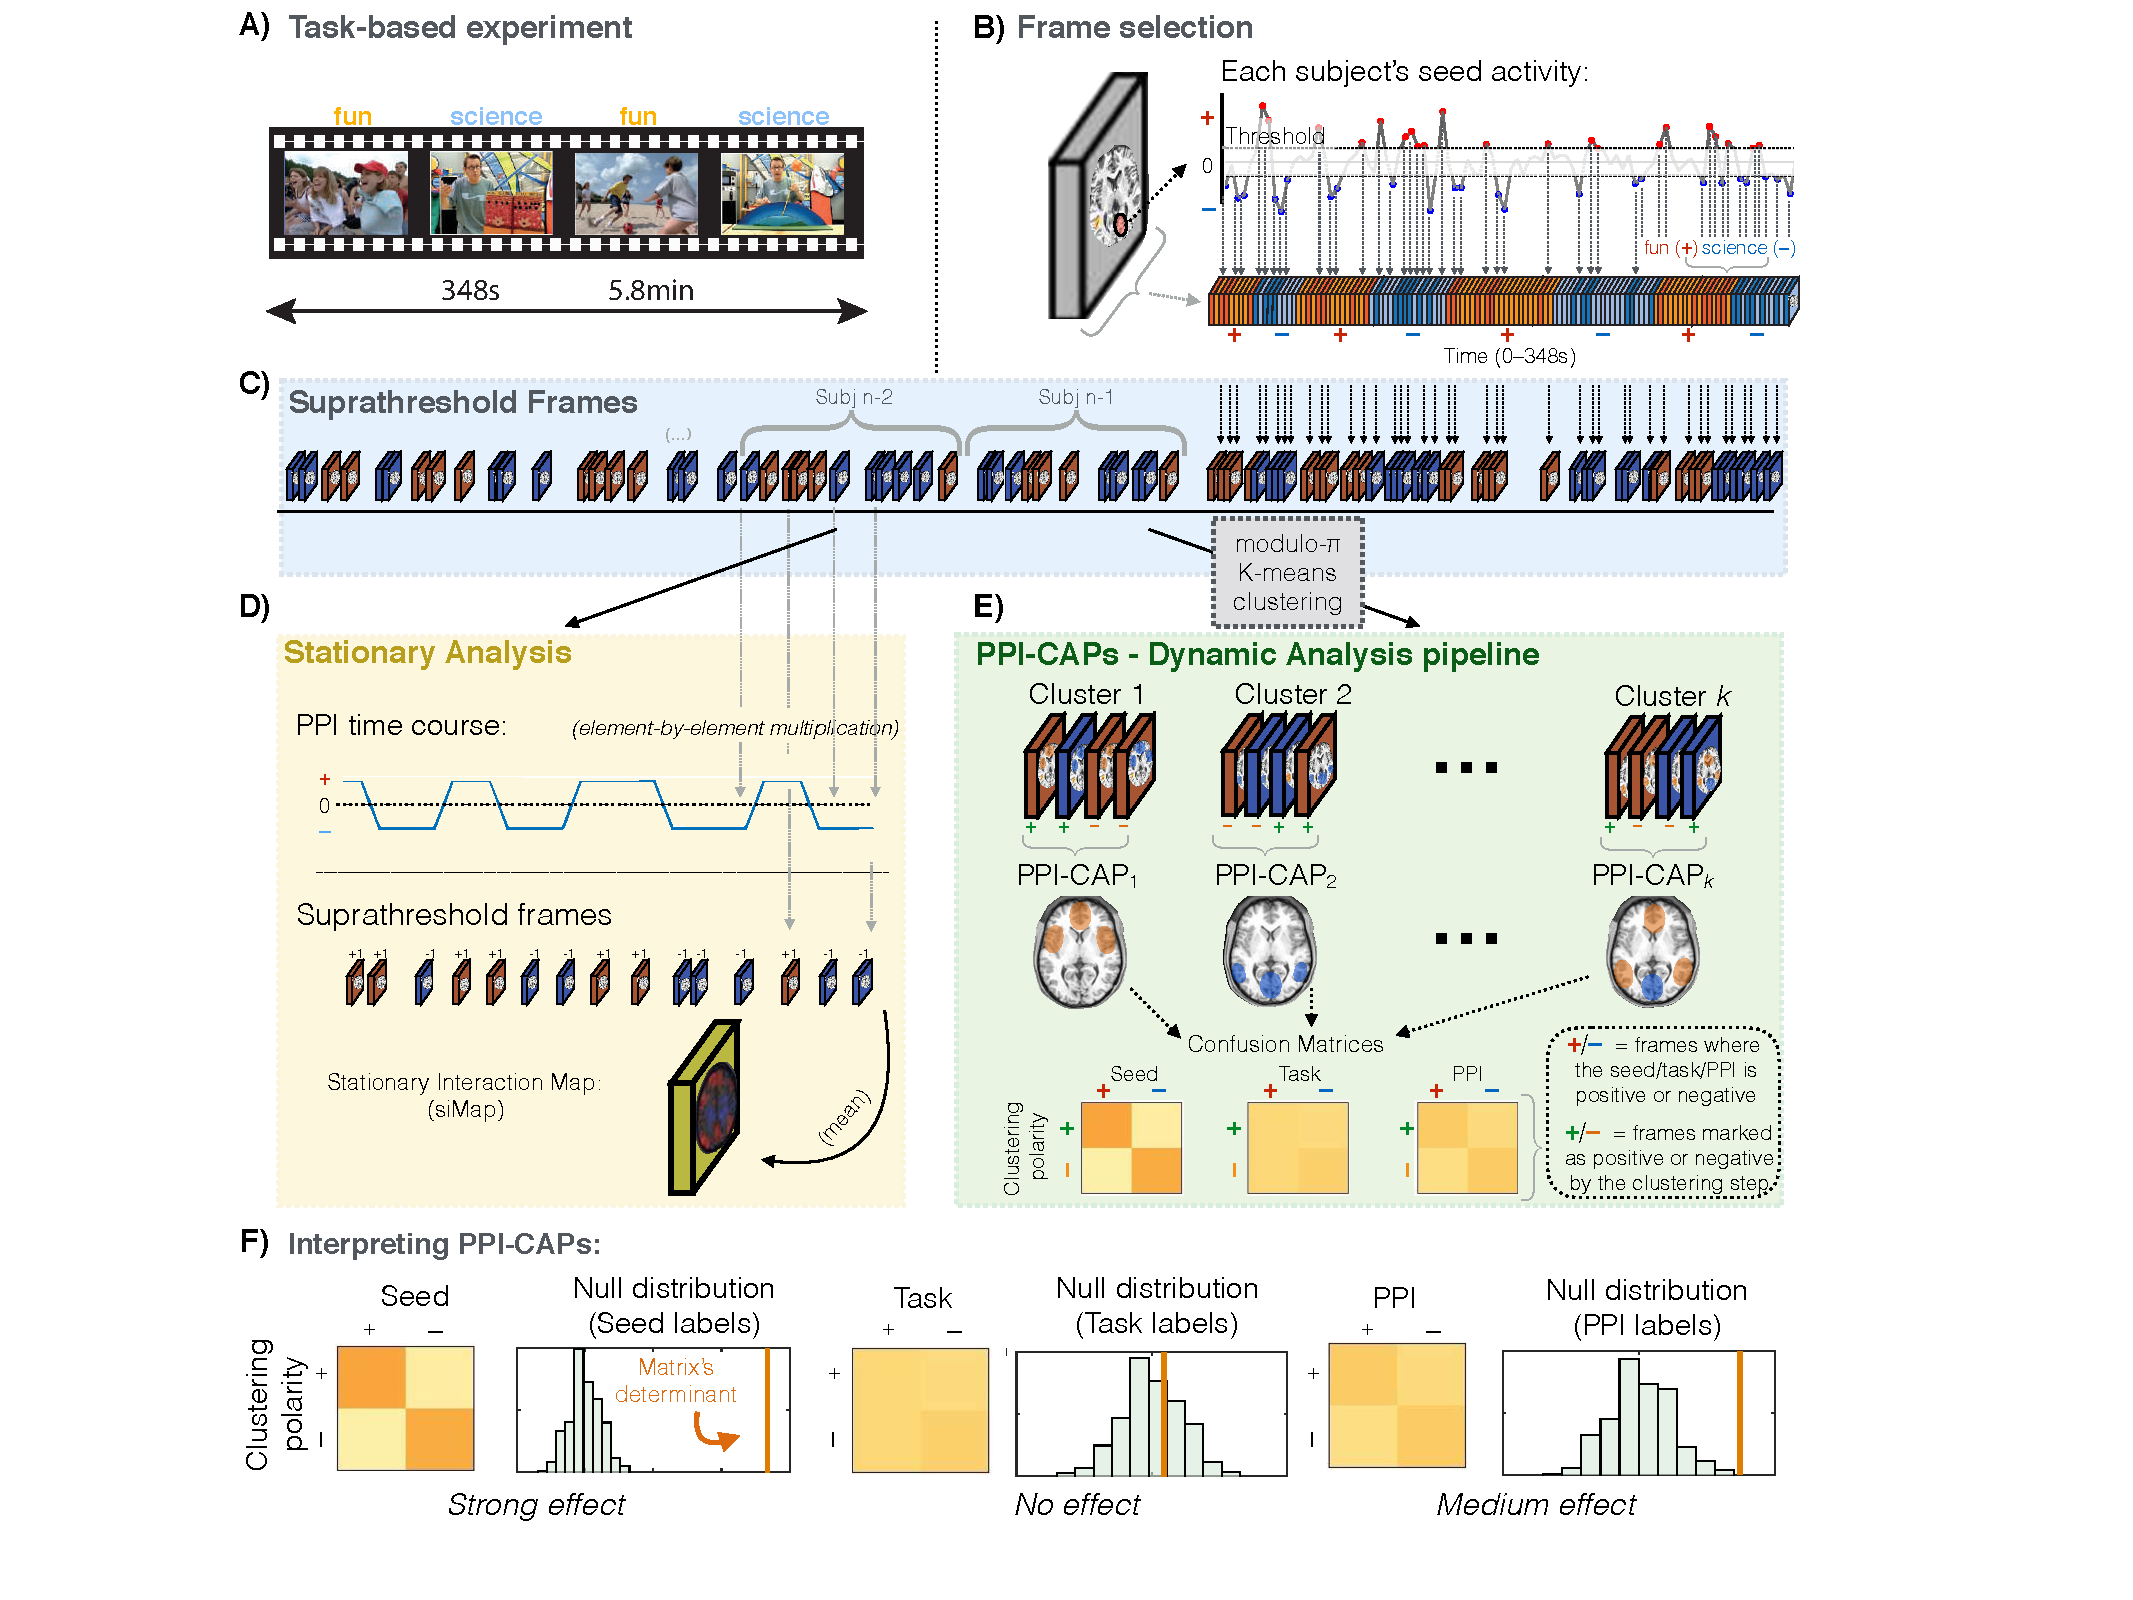
\includegraphics[width=0.95\textwidth]{Ch5/20190927_PPICAPS_Frameworkc}
%\vspace*{-1mm}
\caption{\textbf{The PPI-CAPs analysis pipeline.} A)~We begin with an experimental design containing different task blocks or contexts. Here, we used data acquired in a naturalistic paradigm in which subjects watched a film containing two main types of scenes: \textit{fun} and \textit{science}. B)~For each subject, the z-scored signal from a selected seed is thresholded so that frames in which it is highly active or deactive (darkened in the subject time course) can be considered for further analysis. Orange and blue frames occur during \textit{fun} and \textit{science} scenes, respectively. C)~Suprathreshold frames from all subjects are concatenated. From here on, we can proceed to a static or a dynamic analysis. D)~Static analysis: suprathreshold frames from each condition are multiplied by the sign of the seed and task time courses (which corresponds to the PPI time course) and then averaged, yielding a proxy of the PPI analysis results: the static interaction map, or siMap, at either subject or group level.  E)~Dynamic analysis: suprathreshold frames from all subjects are clustered into a set of PPI-CAPs. Frame labels allow us to count how often a PPI-CAP occurs in each condition in its positive or negative polarity and compare these to the signs of each effect of interest. F)~The frames' polarity after clustering tends to correlate with the sign of the effects it represents. By examining the confusion matrix for each effect (seed, task or PPI), we can determine if a PPI-CAP is strongly related to it (\textit{i.e.}, when the confusion matrix is highly diagonal) or when there is no such effect (\textit{i.e.}, when the confusion matrix has no obvious pattern). }
\label{PPI_CAPs_fw}
\end{figure*}


For the static analysis, we first multiply the selected frames by the sign of the seed and the centred modulating term (\textit{i.e.}, the contrast variable, as it encodes knowledge of the task paradigm) at the corresponding time points. Note that this sequence is equivalent to multiplying the original selected frames by the PPI variable, which corresponds to the multiplication of the sign of the seed and the task time courses. The average of these selected frames leads to a proxy of the conventional PPI results (Figure~\ref{PPI_CAPs_fw}D, bottom), which we refer to as the \textit{static interaction map} (siMap). For a mathematical motivation as well as a toy example that intuitively illustrates this relationship between conventional PPI and static PPI-CAP analyses, we refer to Appendix \ref{appA} and Supplementary Figure~\ref{fig:simapIntuition}, respectively.

For the dynamic analysis, all the originally retained frames are subjected to K-means++ clustering  \citep{Arthur2007} as described in Section \ref{sectionKmeans} (Figure~\ref{PPI_CAPs_fw}E). This step yields PPI-CAPs, their occurrence in time and the polarity of their constituting frames, which allows us to eventually identify meaningful statistics (\textit{i.e.}, effects of task, seed, or their interaction). The next sections further detail the different steps of the pipeline.

\subsubsection{Seed-based frame selection}

The first step of the PPI-CAPs framework is to select a seed region according to prior knowledge about the task being studied or on an exploratory basis---a good discussion on how to choose a seed can be found in \citet{OReilly2012a}. The fMRI frames in which the seed reaches high magnitude values are then selected for further analysis. We refer to frames in which absolute seed activity is above the stipulated threshold as \textit{suprathreshold frames}.

\subsubsection{Static analysis} \label{met:static_analysis}
In the context of point process analyses \citep{Tagliazucchi2012,Liu2013}, simple averaging of selected frames provides a good proxy for seed-based functional connectivity (see Appendix~\ref{appA}), showing that the chosen subset of data contains relevant information. For large datasets, this observation holds for a wide range of thresholds retaining 15\textendash90\% of frames (\citeauthor{Liu2013}, \citeyear{Liu2013}, Figure 1B), while for smaller datasets the threshold must aim at a trade-off between dramatically decreasing the amount of data used for analysis while keeping enough frames to reduce the effects of noise. Note that, besides improving the signal-to-noise ratio, including more frames in the analysis of smaller datasets improves the chance that enough frames will be available for the dynamic analysis.

In a similar validation step, we perform an initial static analysis procedure that can be compared against conventional PPI. Specifically, suprathreshold frames were multiplied by a centred contrast variable---the sign of the PPI regressor, as explained in Section~\ref{sec:methods-ppi-caps}---and subsequently averaged (Figure~\ref{PPI_CAPs_fw}D, yellow inset). Here, we used the strategy described in \citet{Liu2013} to improve the signal-to-noise ratio of an fMRI frame, where a mask was created to cover voxels with the highest 10\% and lowest 5\% values, and all other voxels were set to zero. The spatial correlation between the resulting static interaction map (siMap) and the PPI results is measured using spatial Pearson’s correlation coefficient. This correlation was repeatedly calculated for siMaps including 5\textendash100\% of all frames both at subject and group levels, to test the robustness of the method to the choice of threshold. Since correlation values are range-constrained, when calculating their averages as described in Section \ref{sec:static_analysis} and shown in Figure~\ref{fig:PPI_CAPs_Fig2}C we first applied Fisher's z transform (the inverse hyperbolic tangent) to all Pearson's r values \citep{Cox2008}. After calculating the means, we then converted the results back to Pearson's r values by calculating the former's hyperbolic tangent. For the group maps, z-scored seed activations were calculated for all subjects, whose data were concatenated and frames selected as per individual subjects.    The PPI analysis was performed using the standard procedure from  SPM8 where three regressors are included in a general linear model design, relating to the time courses of the PPI, the seed, and the task, respectively. Note that the PPI regressor in SPM is derived by deconvolving the haemodynamic response function (HRF) from the seed time course, multiplying the latter by the task time course, and then reconvolving the final series with the HRF. The exact same task time course and seed region were used for both analyses.

\subsubsection{Dynamic analysis} \label{sectionKmeans}
For a dynamic analysis of brain function during task, we identify the PPI-CAPs that may present a seed, task, or interaction effect (Figure~\ref{PPI_CAPs_fw}E). To this end, we applied  K-means++ clustering on the suprathreshold frames of all subjects, using a \textit{modulo-$\pi$} cosine distance as a similarity measure, which we have named as such because it consists in the following: frames among which only the signs of the voxels were reversed were considered to be representations of the same pattern, with opposite polarity (\textit{e.g.}, if frame \textit{a} showed an active prefrontal cortex and deactive occipital cortex, while frame \textit{b} displayed a deactive prefrontal cortex and active occipital cortex, then, assuming {$\mathbf{F}_a$} and {$\mathbf{F}_b$} are the frames' voxel patterns, {$\mathbf{F}_a$} $\approx$ -{$\mathbf{F}_b$}). 

Traditionally, the iterative algorithm to implement K-means consists of two steps: 1) assigning each data point to its closest centroid given the defined similarity metric \textit{d}; 2) updating the centroids according to their assigned data points (\textit{e.g}., by updating each centroid with the average of the normalized data points most recently assigned to it). At each iteration, the cluster label assigned to the $i^{th}$ frame, $\mathbf{L}_i$, is given by:
 \begin{equation} \label{eq:labelassigment}
 \mathbf{L}_i = \argmin_{\kappa} \big( \text{d}( \mathbf{C}_\kappa, \mathbf{F}_i )  \big)\text{,}
 \end{equation}
 where $\kappa$ runs over the number of clusters, $\mathbf{C}_\kappa$ is the value of the $\kappa^{th}$ cluster's centroid, $\mathbf{F}_i$ is the voxelwise activation pattern for the $i^{th}$ frame, and \textit{d} is the selected distance metric.
 
 
 
 To add information regarding the frame polarity in PPI-CAPs, in our approach we set \textit{d} to be the \textit{modulo-$\pi$} cosine distance (mpcos):
 \begin{equation}
 \label{eq:mod-pi-cos-dist}
 d(\mathbf{x},\mathbf{y}) =\mathrm{mpcos}(\mathbf{x},\mathbf{y}) = 1 -  \left|  \frac{ \mathbf{x} \cdot  \mathbf{y}}{\|\mathbf{x}\| ~\|\mathbf{y}\|} \right|,
 \end{equation}
 where $  \mathbf{x} \cdot \mathbf{y} = \sum_k x_k y_k  $ is  the standard inner product and the norm is $\| \mathbf{x} \|= \sqrt{\mathbf{x} \cdot \mathbf{x}}$. The polarity $P_i$ of  frame $F_i$ is thus equivalent to sign($  \mathbf{C}_\kappa \cdot \mathbf{F}_i $). From here on, we will describe frames for which $P_i = 1$ as having a ``positive polarity", and those for which $P_i = -1$ as having a ``negative polarity". Note how the metric in equation~\eqref{eq:mod-pi-cos-dist} compares to the standard cosine distance, given by:
 
 \begin{equation}
 \cos(\mathbf{x},\mathbf{y}) = 1 -  \frac{ \mathbf{x} \cdot  \mathbf{y}}{\|\mathbf{x}\| ~\|\mathbf{y}\|} ,
 \end{equation}
meaning that \textit{modulo-$\pi$} cosine implies no additional complexity as compared to the standard cosine distance metric.
 The value of each centroid $\mathbf{C}_\kappa$ is then updated as such:
\begin{align}\label{eq:centroid}
\mathbf{C}_\kappa &= \frac{1}{N_\kappa} \sum_{i=1}^{N_\kappa} P_i \frac{\mathbf{F}_i}{\|\mathbf{F}_i\|}\text{,} 
\end{align}
where $N_\kappa$ is the number of frames in the $\kappa^{th}$ cluster and $\|\mathbf{F}_i\|$ is the magnitude of frame $\mathbf{F_i}$.

The final cluster centroids then form the PPI-CAPs.
Each frame is thus annotated according to: 1)~the time point it corresponds to; 2)~the task or condition label which corresponds to that time; 3)~the subject to whom it belongs; and 4)~the polarity in which it occurred (positive or negative). This information can then be used to investigate differences in PPI-CAP occurrence across settings. 

\subsubsection{Significance assessment}
If a PPI-CAP has a strong main or interaction effect, the polarity of the frames that constitute it will tend to correlate with the sign of that effect for the same time points. To visualise if this is the case, we can thus generate confusion matrices for each effect and PPI-CAP. When there is a strong correlation, the higher values of a confusion matrix will tend to load on one of its diagonals, and the relevance of this relationship can be measured by taking the matrix's determinant, which we will call the \textit{det-index}. To test whether this value is significant, we can thus generate a null distribution by performing random permutations of the effect of interest's labels and re-calculate the det-index each time. Finally, we see where the real det-index stands in the distribution (Figure~\ref{PPI_CAPs_fw}F).
For the results shown here, we performed 3000 random permutations for each test. We disclose the uncorrected p-values and indicate the significance level that should be used to correct for multiple corrections, controlling for the number of PPI-CAPs.


\subsubsection{Choosing the number of PPI-CAPs}
Effective Connectivity methods such as PPI provide a summary spatial map of task-specific seed relationship modulation. To disentangle which and when instantaneous patterns of activity support the summarized PPI findings, we must first determine the number of clusters into which to categorize the data. To this end, we employed Consensus Clustering \citep{Monti2003}. This approach applies K-means clustering on several subsamples of the data and calculates the \textit{consensus matrix} $\mathcal{M}$. Each element $\mathcal{M}(a,b)$ indicates the fraction of subsamples in which two frames $a$ and $b$ were both retained and clustered together. The optimal number of clusters can then be inferred by visual inspection of the ordered matrix $\mathcal{M}$, as well as of the cumulative distribution function (CDF) of $\mathcal{M}$  for different values of $k$.  

Additionally, for every $k = {3,4,...,8}$ we calculated the number of frames from each subject that contributed to each of the $k$ PPI-CAPs.
This helped us choose a $k$ value for which the distribution of PPI-CAPs across subjects was roughly uniform. We applied consensus clustering for $k = {3,4,...,8}$ using 10 random subsamples for every $k$. Each subsample included 80\,\% of the suprathreshold frames of all subjects, and K-means was computed for 50 random initialisations for each subsample.
To obtain the final clustering result, we applied K-means clustering with the optimum $k$ on 100\,\% of the suprathreshold frames and kept the best result from 50  random initialisations, \textit{i.e.}, the one that minimised the total sum of modulo-$\pi$ cosine distances between frames and centroids.

\subsubsection{Experimental data}

To validate the method, we used fMRI data from 16 healthy subjects (mean age $22.92 \pm 8.14$ years) watching a short TV program about the effects of sun exposure. The video alternated between two contexts: 1) images of several children playing by the beach (from here on described as \textit{fun}); 2) scenes where scientific concepts were explained in a laboratory (we will call this context \textit{science}). The movie can be watched online\footnote{\url{https://miplab.epfl.ch/index.php/miplife/research/supplement-asd-study}}, and a detailed description of the dataset can be found in \cite{Jochaut2015}. One subject was excluded due to high motion for having $>$25\% of frames with framewise displacement (\citeauthor{Power2010}, \citeyear{Power2010}) higher than 0.5~mm. Thus, 15~subjects were analysed (mean percentage of scrubbed frames = 2.2\%, SD = 5.8\%). 179~volumes (Tim-Trio; Siemens, 40 transverse slices, voxel size = 3~mm $\times$ 3~mm $\times$ 3~mm; repetition time~=~2000~ms; echo time = 50~ms; field of view = 192) were available per subject, as well as an anatomical T1-weighted rapid acquisition gradient echo sequence (176 slices, voxel size = 1 mm $\times$ 1 mm $\times$ 1 mm, field of view = 256), acquired at the end of the scanning. All participants have given their written informed consent, which was approved by the local ethics committee (Biomedical Inserm protocol C08–39).

\subsubsection{fMRI preprocessing}
Functional images were preprocessed using SPM8 (Wellcome Department of Imaging Neuroscience, UK) where they were realigned to correct for head motion; coregistered with structural images; normalized  in the Montreal Neurological Institute (MNI) stereotactic space; and spatially smoothed using a 6~mm full width at half maximum isotropic Gaussian kernel. In order to remove haemodynamic temporal blurring and better approximate neural activity, blood oxygenation level-dependent (BOLD) signals were deconvolved with the canonical haemodynamic response function from SPM8. This was done using an implementation of the Wiener filter from spm\_peb\_ppi.m, an SPM8 function that computes BOLD deconvolution in the context of PPI analyses. Voxels were then z-scored in time \citep{Liu2013}.


\subsubsection{Considerations for the application of PPI-CAPs}
We applied PPI-CAPs on a movie-watching dataset to illustrate its potential to uncover task-related time-resolved effective connectivity in a realistic setting. To this end, the posterior cingulate cortex (PCC) was selected as a seed region for this study due to its well documented connectivity arrangements \citep{Lin2017} and description as a hub region \citep{Andrews-hanna2010}. A previous study by our group on transient brain activity also revealed the PCC as the node with the most spatial overlap between networks \citep{Karahanoglu2015a}. We used SPM8's Check Orthogonality tool to understand how collinear the PCC activity was with our task paradigm, MATLAB's Skewness function to check that the activity was not skewed, and we verified that the magnitude of the seed time course did not correlate with the sign of the task (Supplementary Material \ref{fig:seedcheck}). To keep in line with previous work that inspired our method \citep{Liu2013}, we report the thresholding step based on the percentage of data points kept for the dynamic analysis. As discussed later, PPI-CAPs is robust to a very wide range of seed activity thresholds for selecting frames to retain for analysis. For the results presented here, we use 60\% of the available frames as a trade-off between optimising data usage from our dataset and obtaining clear brain patterns in the dynamic analysis, avoiding noise that is not averaged out due to a lack of frames in some PPI-CAPs.



%----------------------------------------------------------------------------------------
%	RESULTS
%----------------------------------------------------------------------------------------
\subsection{Results}

\subsubsection{Static analysis} \label{sec:static_analysis} 

\paragraph{Single subject level: }  
At a single subject level, the spatial pattern from the corresponding siMap, generated as the average of the 60\% suprathreshold fMRI frames (when the PCC seed was highly active), was  reasonably correlated with the resulting map from a 1\textsuperscript{st} level PPI Analysis (average spatial correlation: \textit{r}=0.76 $\Mypm$ 0.28). This was the threshold we chose in order to keep enough frames for the dynamic analysis, but the similarity was robust to the choice of threshold for frame selection across subjects (Figure \ref{fig:PPI_CAPs_Fig2}C): correlation was already high even when only 15\% of  suprathreshold frames were kept (\textit{r}=0.71 $\Mypm$ 0.1). To further illustrate that the correlation strength remains stable for varying cutoff values, we first calculated the mean subject-level Fisher's z-transformed correlations (see Section \ref{met:static_analysis}) for each threshold that kept from 15 to 60\% of original frames. Then, we computed the average of these means and transformed it back to Pearson's r, for which we obtained 0.76 with SD$\pm$0.04. The correlation gradually drops when fewer than 15\% of the frames are used, which is expected as not enough frames are selected to average out the noise. 

\begin{figure*}[t]
\centering
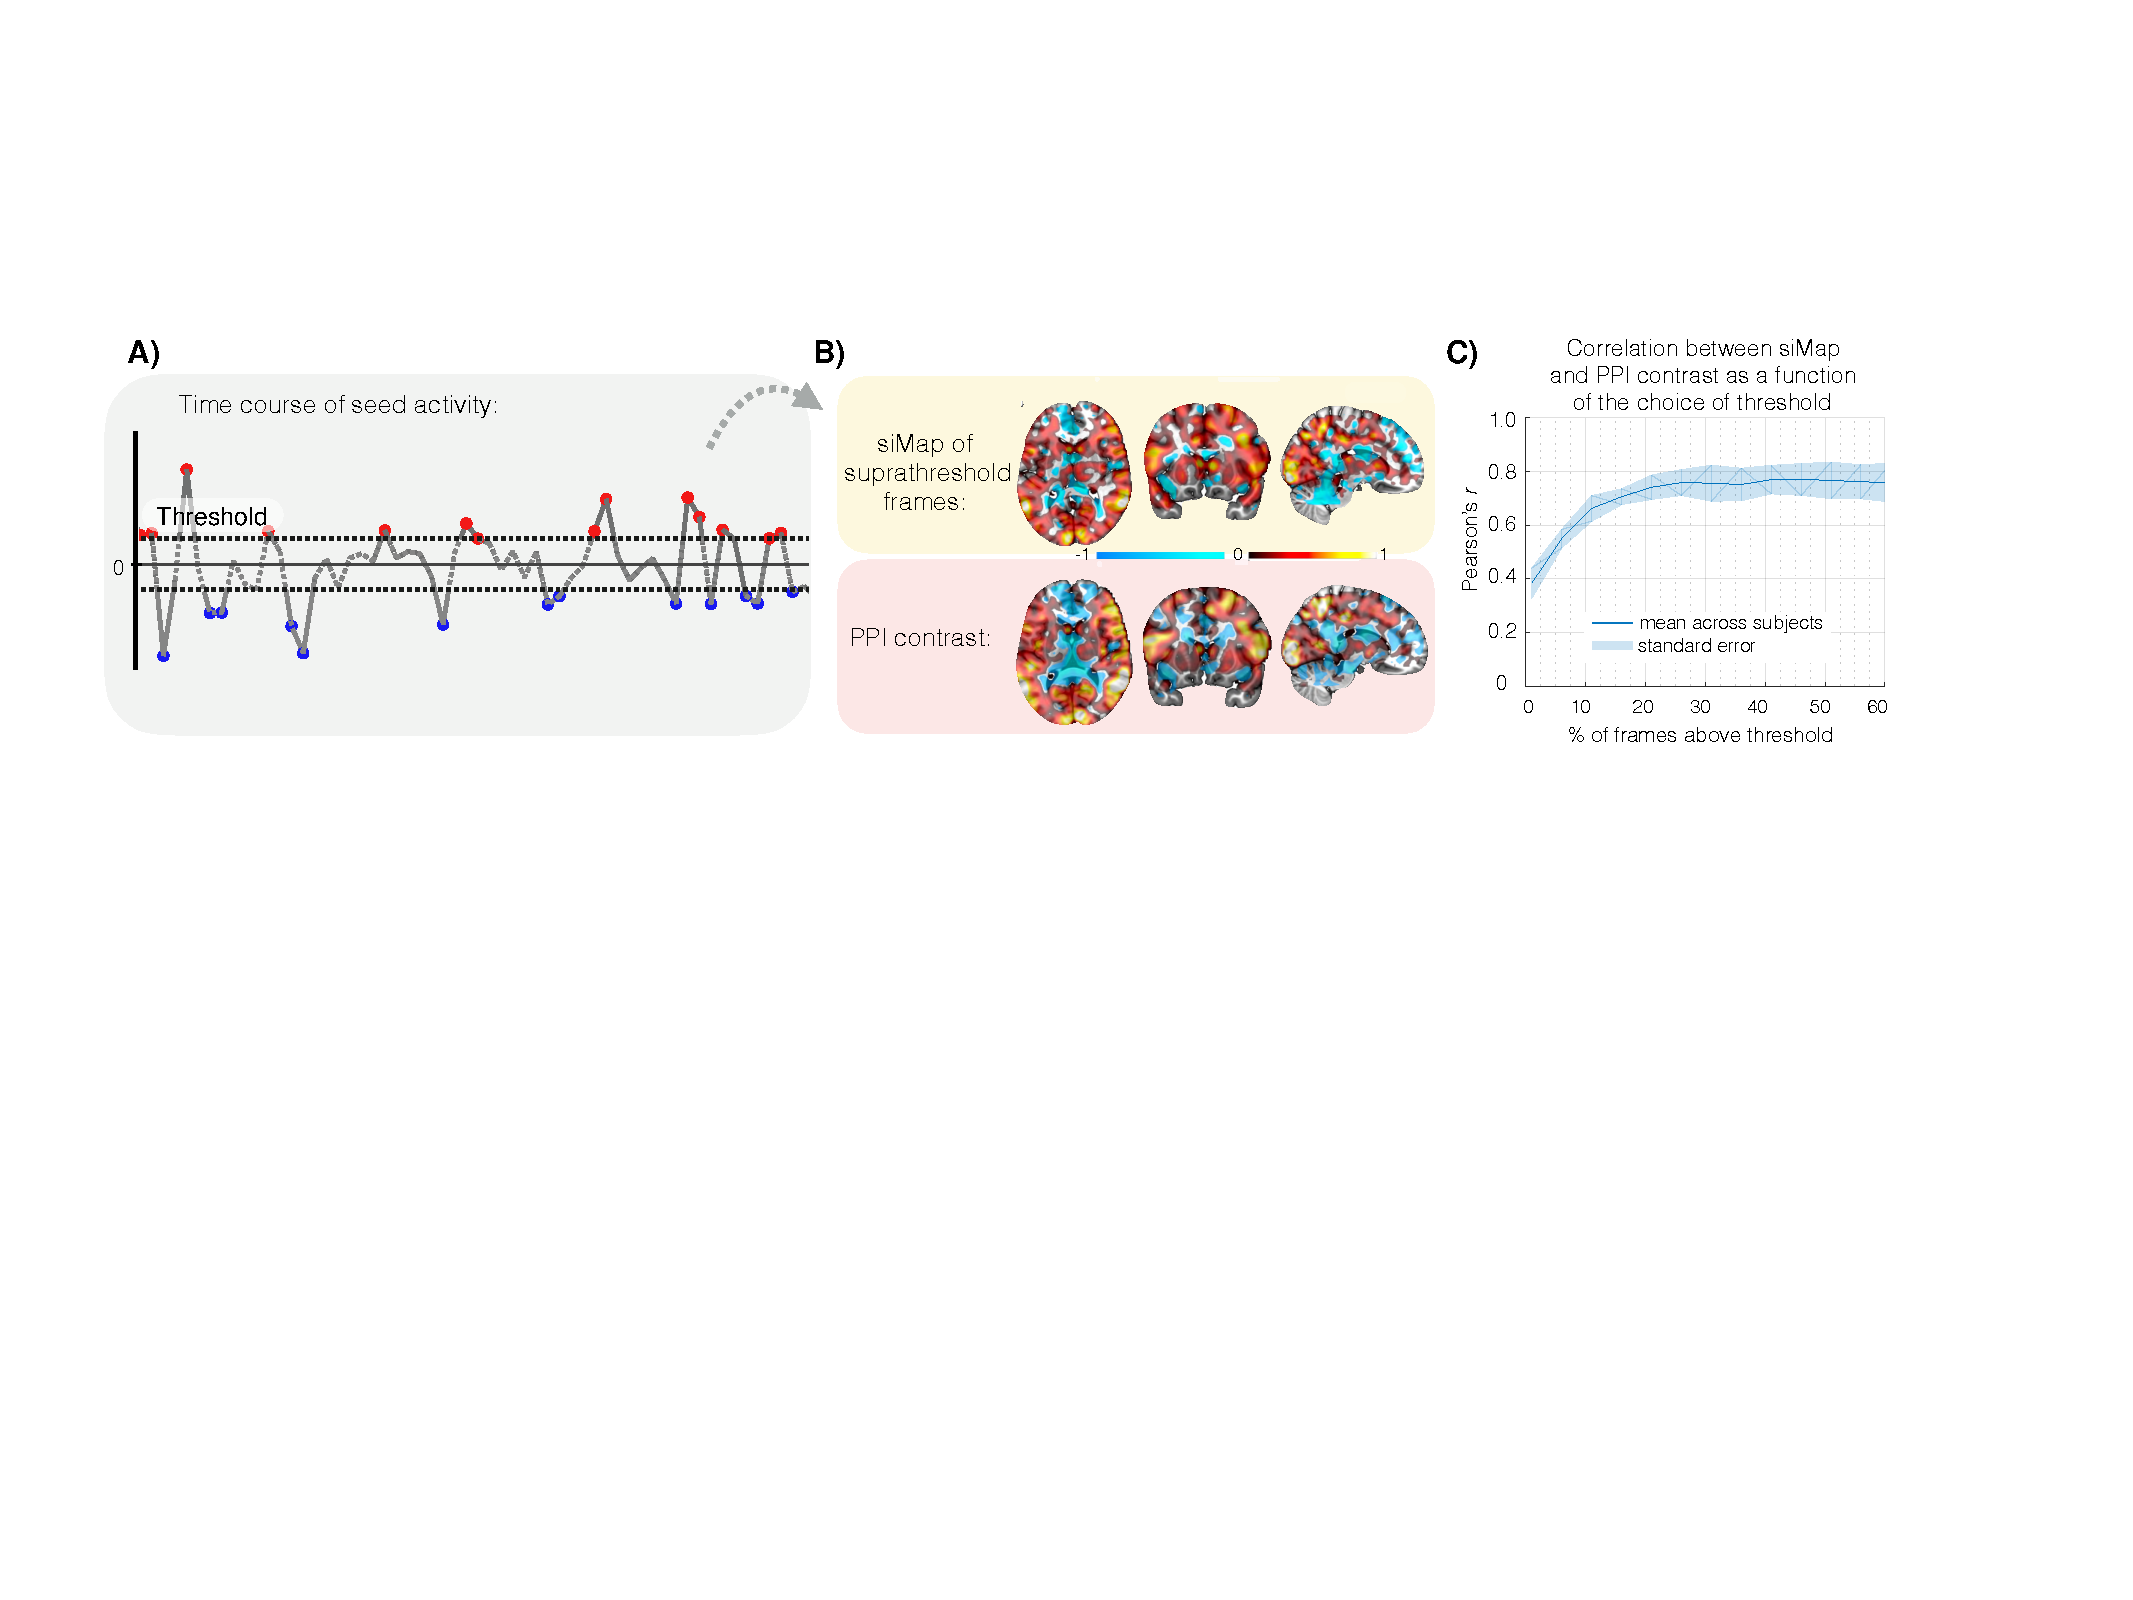
\includegraphics[width=1\textwidth]{Ch5/20191125_Fig2c}
%\vspace*{-9mm}
\caption{\textbf{The static interaction Map (siMap) using a subset of fMRI frames accords with the PPI contrast obtained from all the available data.} A) Frames from time points when the considered seed is highly active are selected. A fraction of seed time course is shown for one subject. B) Retained frames are then multiplied by the PPI variable and averaged, yielding the static interaction map (siMap), as shown for the same subject with a yellow background. For comparison, the contrast map resulting from a PPI analysis using all frames is also shown with a red background. C) The siMap and PPI contrast map are reasonably correlated (\textit{r} $>0.7$) even when the former is computed using only 15\% of the frames, and this similarity remains high as more frames are used, showing that the selection of relevant frames is robust to the choice of threshold. The dark blue curve represents the average correlation between the siMap and 1\textsuperscript{st} level PPI contrast map across subjects, and the light blue shading denotes the standard error. The correlation means were calculated by averaging Fisher's z transforms of the Pearson's r values, and transforming the result back to Pearson's r.}
\label{fig:PPI_CAPs_Fig2}
\end{figure*}



\paragraph{Group level: } At the group level, the spatial pattern from the siMap obtained using 60\% of frames also correlated (\textit{r}~=~0.85) with the  pattern obtained from a 2\textsuperscript{nd} level PPI analysis (Supplementary Figure~\ref{fig:groupSimap}), which showed a significant increase in effective connectivity between the PCC and the right V5 during \textit{fun} scenes (height threshold T~=~3.8, p~$<$~0.001; right V5 MNI coordinates x~=~39, y~=~-67, z~=~-2; cluster size~=~185 voxels;  p\textsubscript{fwe-corr}~$<$~0.001). 

Together, these results demonstrate that even a subset of fMRI frames, selected when the seed activity is highly active or strongly deactivated, contains relevant information about how its co-activation with other regions changes based on task context.



\subsubsection{Dynamic analysis} 

\paragraph{Choice of number of clusters} An analysis of PPI-CAP occurrences for  $k={3,4,...,8}$ showed that for $k\geq 6$, some patterns never occurred in some subjects, while $k=4$ and $k=5$ were the cases with the most homogeneous distribution of pattern occurrence per subject (see Supplementary Fig.~\ref{fig:consensus}). Visual inspection of the consensus matrices showed that the most stable values for $k$ (\textit{i.e.}, the values for which any two frames would most consistently be clustered together or separately) were $k=3$ and $k=4$. Taking these observations together, we proceeded with the analysis generating 4 clusters, as this $k$ value combined the beneficial features of: 1) yielding PPI-CAPs that are homogeneously distributed across subjects; 2) being highly stable (\textit{i.e.}, running the clustering several times would always produce similar results); and 3) representing a reasonable balance between variety and redundancy \citep{Liu2013}.



\paragraph{Temporal decomposition of psychophysiological interactions into co-activation patterns} Our dynamic analysis revealed four recurring patterns of co-activation (Fig.~\ref{fig:PPI_CAPs_Fig3}A), all of which were significantly modulated by the seed, the context or an interaction between the two (PPI effect) after correcting for multiple comparisons (significance level $\alpha$ \textsubscript{$0.05/4$} = 0.0125). 
PPI-CAP\textsubscript{1} includes nodes of the visuospatial (VSN) and attention (AN) networks correlated with the PCC and nodes of the fronto-parietal network (FPN) and salience networks (SN) anti-correlated with the PCC (p~$=$~0.008). Additionally, the VSN and AN had a tendency to be more active, while the FPN and SN were more deactive,  during \textit{science} scenes as compared to \textit{fun} ones (p~=~0.019). PPI-CAP\textsubscript{2} combines the FPN correlated, plus the posterior insula and visual nodes anti-correlated, with the seed (p~$=$~0.0009). PPI-CAP\textsubscript{3} corresponds to the default mode network (DMN) and was significantly correlated with the seed (p~$=$~0.0009). It also appeared more often during \textit{fun} scenes rather than \textit{science} ones (p~=~0.008). PPI-CAP\textsubscript{4}, in turn, which contains the V5 and nodes of the VSN, showed not only a significant seed effect (p~$=$~0.0009), but also a PPI effect (p~$=$~0.0009).  Supplementary Figure~\ref{fig:PPI_CAPs_Fig5} shows the exact times where each PPI-CAP appeared more consistently in their positive---or negative (meaning that the signs of the voxels should be flipped)---configuration across subjects, and  Supplementary Figure~\ref{fig:permanova} shows their corresponding permutation histograms. 


\begin{figure*}[t!]
\centering
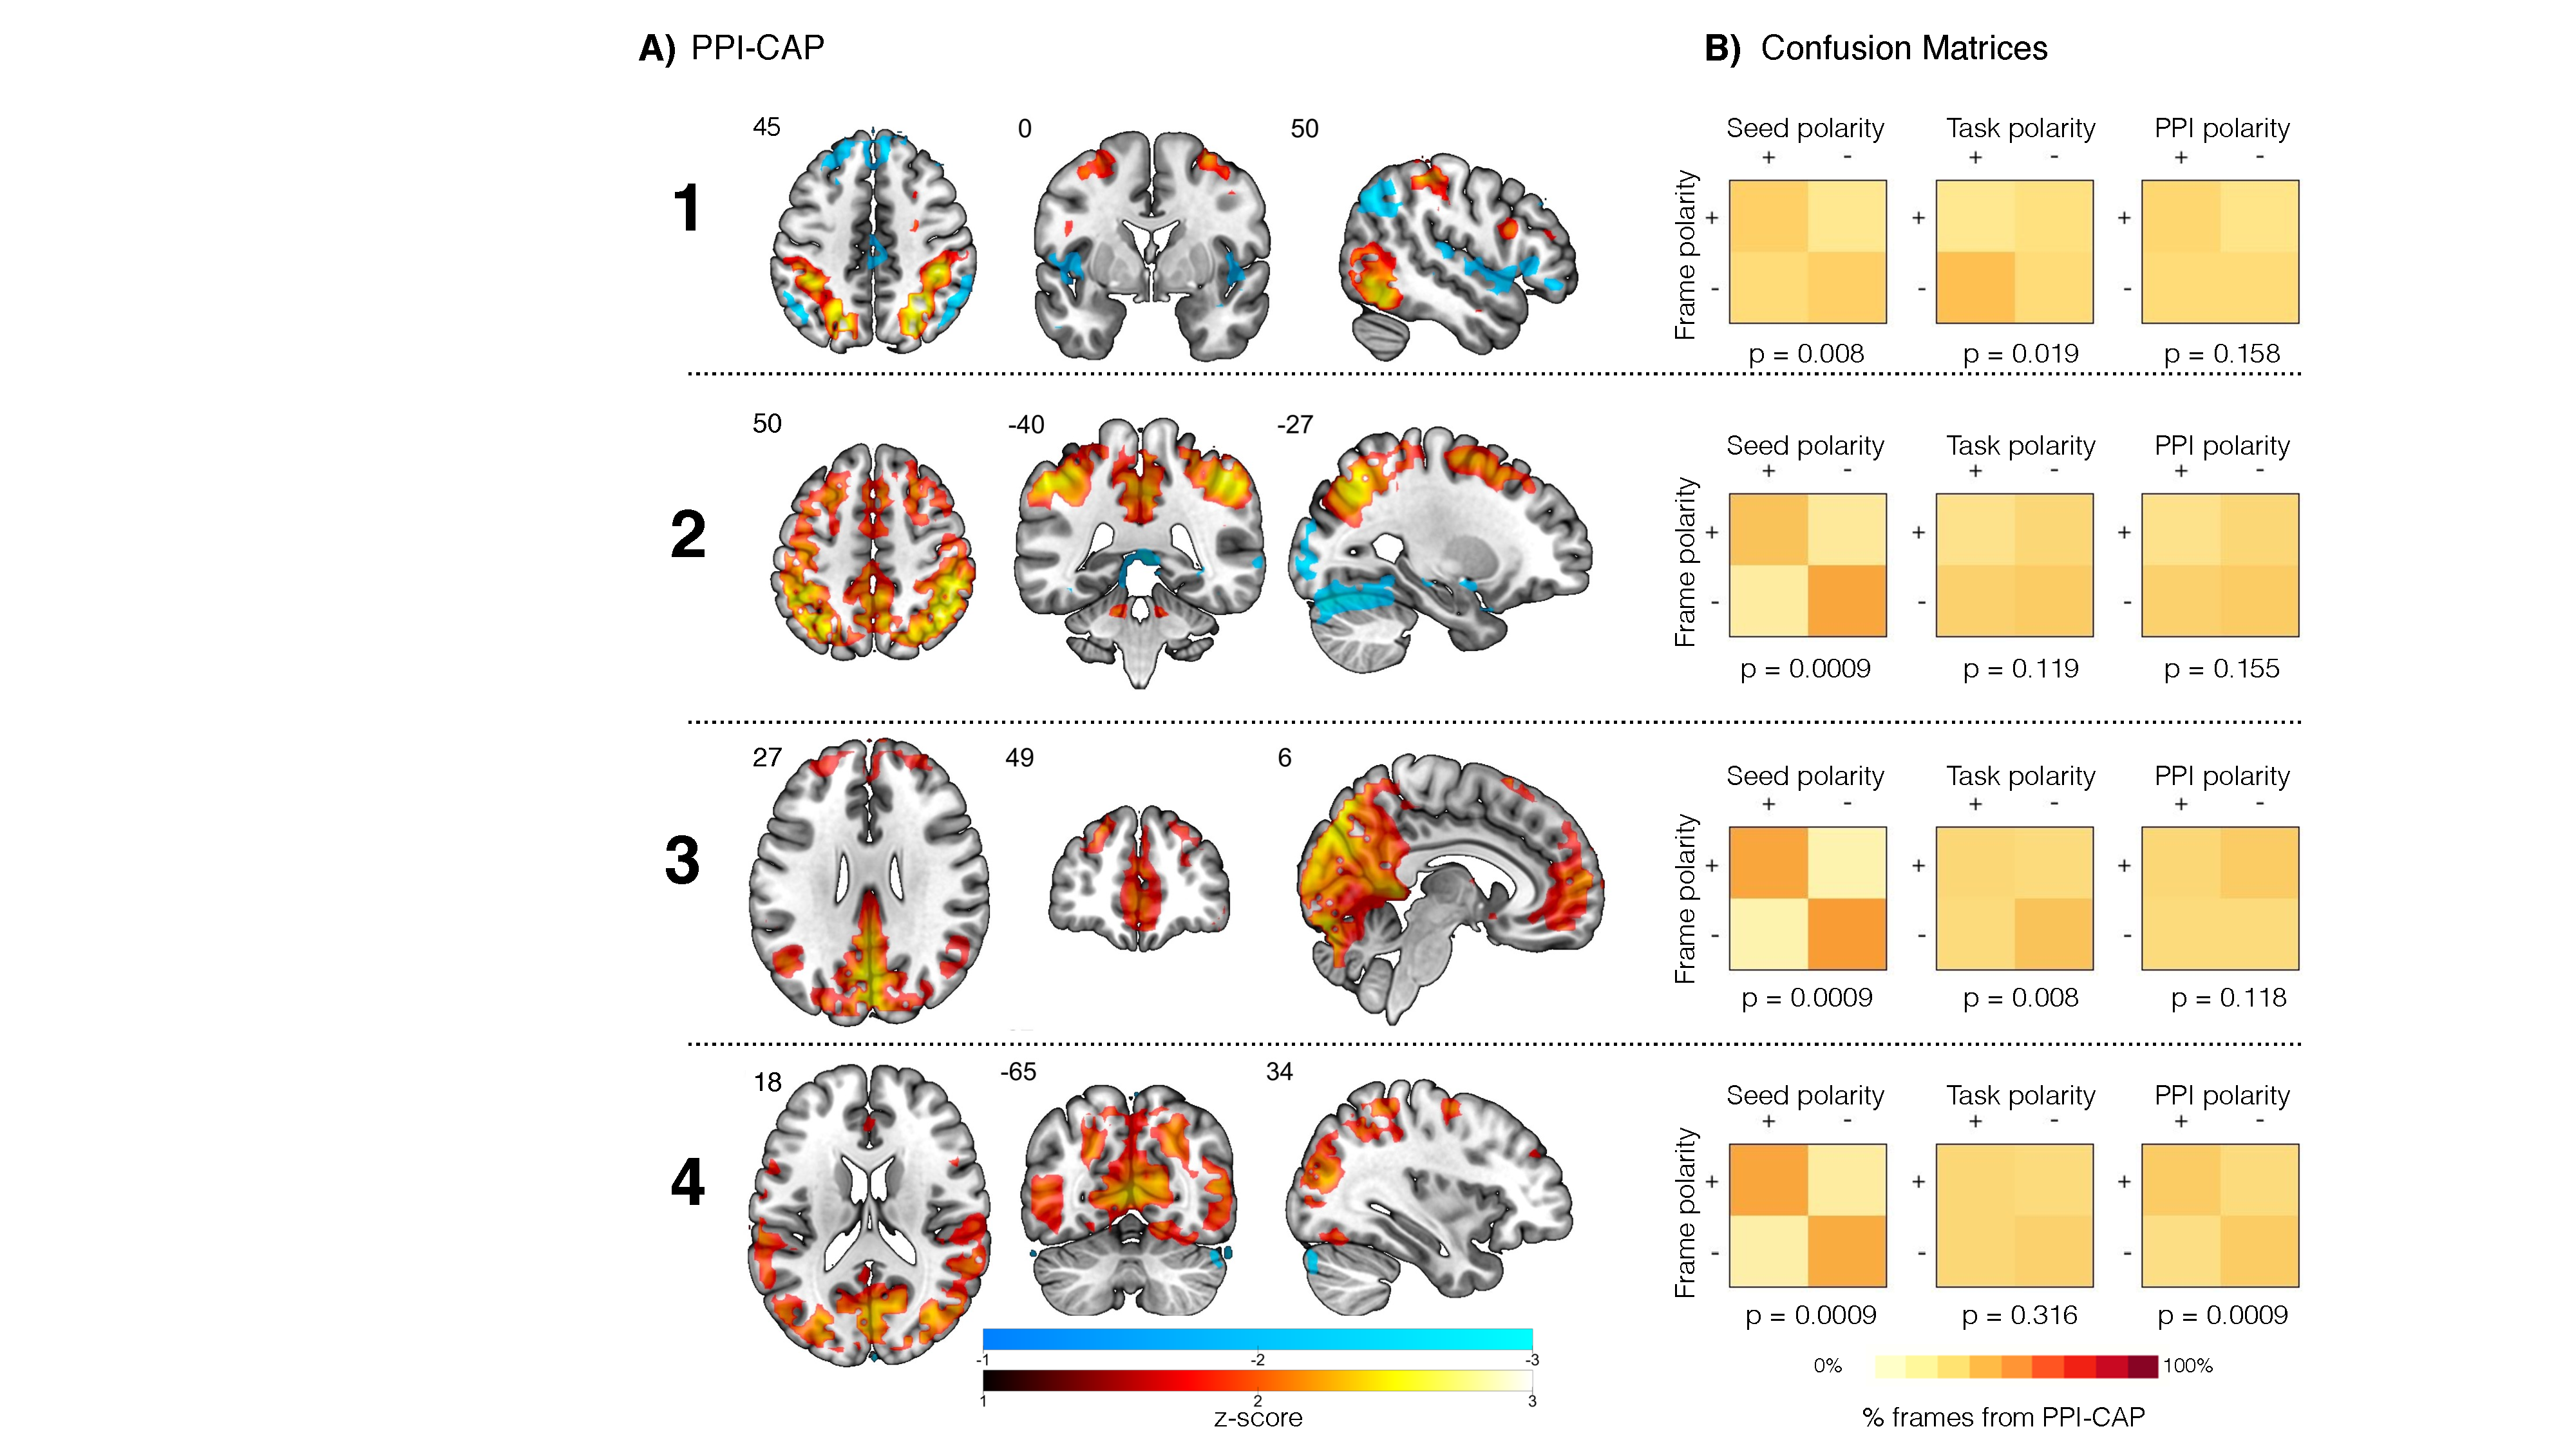
\includegraphics[width=1\textwidth]{Ch5/20191120_PPI_CAPs_Fig3}
\vspace*{-3mm}
\caption{\textbf{PPI-CAPs reveal patterns of co-activation that have a seed; task; or an interaction effect.} A) We retrieved four PPI-CAPs from the Movie Watching dataset by clustering suprathreshold frames: PPI-CAP\textsubscript{1} includes activated visuospatial and attention networks and deactive nodes of the fronto-parietal network (FPN) and salience networks; PPI-CAP\textsubscript{2} includes an activated FPN plus deactive posterior insula and visual nodes; PPI-CAP\textsubscript{3} corresponds to nodes of the default mode network; and PPI-CAP\textsubscript{4} contains the V5 and visuospatial network. B)~Confusion matrices depict how closely the polarity of the frames that make up each PPI-CAP relate to the sign of each effect. A clear diagonal (or anti-diagonal) pattern indicates a strong effect. All PPI-CAPs show a significant seed effect, PPI-CAP\textsubscript{3} shows a significant task effect, and PPI-CAP\textsubscript{4} shows a significant PPI effect, after Bonferroni correction for the number of PPI-CAPs. Raw p-values reported below the corresponding confusion matrices.}
\label{fig:PPI_CAPs_Fig3}
\end{figure*}



\paragraph{Consistency of PPI-CAPs across subjects and brain activity decoding} Our time-resolved method allowed us to investigate how consistent each PPI-CAP was across subjects and throughout the experiment. Figure~\ref{fig:PPI_CAPs_Fig4} illustrates this analysis for PPI-CAP\textsubscript{4}. By inspecting moments when the PPI-CAP appeared consistently for several subjects, we were able to identify specific video frames that elicited the co-activation pattern. For PPI-CAP\textsubscript{4},  moments of positive activation, that is, moments when the V5 and visuospatial network were more active, corresponded to scenes in which there was high motion (\textit{e.g.}, a group of children playing football), whereas a negative polarity of this pattern was related to moments of stillness (Figure~\ref{fig:PPI_CAPs_Fig4}).
Supplementary Figure \ref{fig:PPI_CAPs_Fig5} shows these results for all four PPI-CAPS: for PPI-CAP\textsubscript{1}, moments of positive polarity corresponded to scenes in which the main object (or character) was zoomed into and movements were slow, whereas a negative polarity (meaning a negative VSN and AN, with activated FPN and SN) was related to moments when some goal-oriented action was being performed. For example, at 1'38'', while a group of children are sat at the beach, one of the girls is clearly reaching out for sand to build her castle.   PPI-CAP\textsubscript{2} seemed to be more strongly active during moments when there are lots of people on the scene, and more consistently negative (\textit{i.e.}, deactivated FPN and activated posterior insula) when the scene changes to only one person on screen, explaining concepts about the danger of sun exposure. PPI-CAP\textsubscript{3} appeared more with a positive polarity during zoomed-out scenes where many people were present and interacting, or when science concepts had been explained for a while in the laboratory scenario. These results illustrate PPI-CAPs' ability to link a pattern's occurrence to specific moments of the experimental paradigm.


\begin{figure*}[h!]
\centering
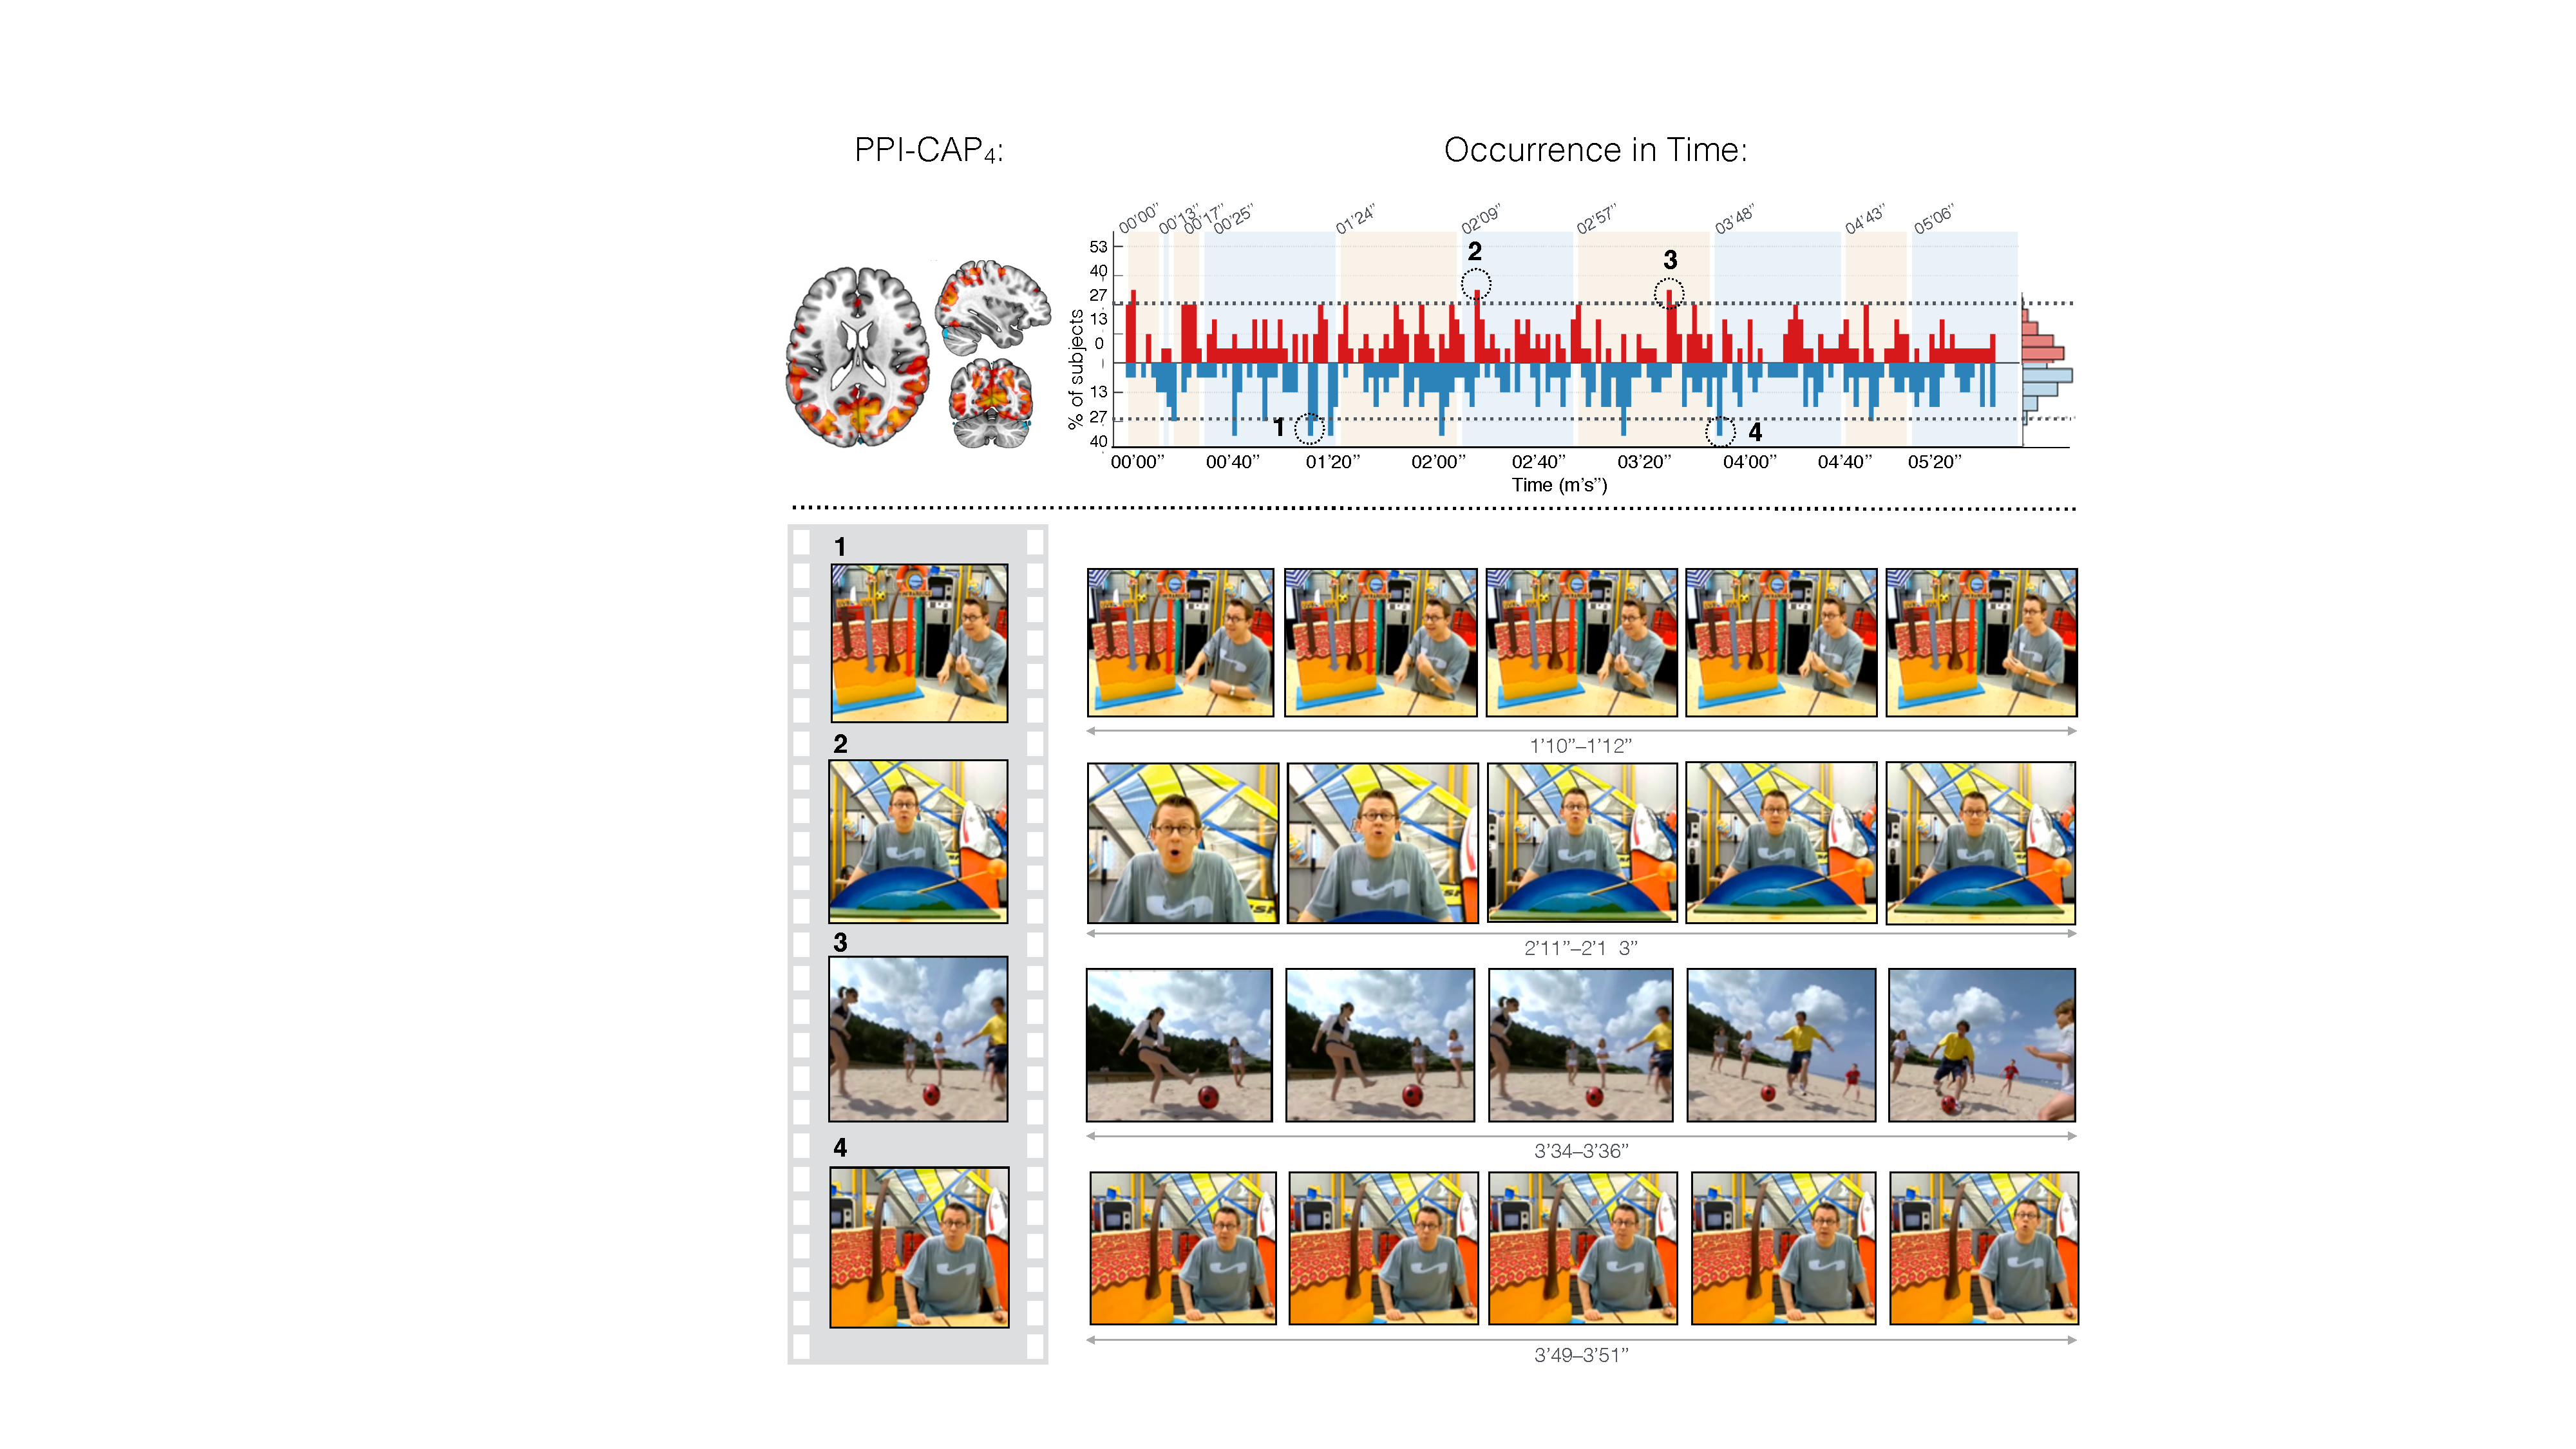
\includegraphics[width=1\textwidth]{Ch5/20190809_PPI_CAPs_Fig4}
%\vspace*{-3mm}
\caption{\textbf{PPI-CAPs enables the time-resolved analysis of  effective connectivity consistency across subjects.} For PPI-CAP\textsubscript{4}: (Top) The plot shows the percentage out of all 15 participants (y-axis) of subjects for whom this PPI-CAP was present at each fMRI frame (x-axis). Red and blue bars indicate the percentage for appearances in positive and negative configurations, respectively. Orange and blue background patches correspond to \textit{fun} and \textit{science} scenes, respectively. The histogram on the rightmost side of the top panel depicts the distribution of random consistency across subjects for each polarity, calculated by randomly permuting the time points on which the PPI-CAP appeared for each subject, then re-calculating the subject consistency across time. The dashed line represents the value of the 99\% percentile from the random distribution, indicating that a subject consistency above this threshold is significant. Four sample time points of high consistency were highlighted. Numbers above the brain slices correspond to MNI coordinates. (Bottom) Video frames spanning a duration of 2~seconds, centred at each frame which corresponds to the timing of high consistency indicated in the top plot. For other PPI-CAPs see Supplementary Figure \ref{fig:PPI_CAPs_Fig5}.  }
\label{fig:PPI_CAPs_Fig4}
\end{figure*}



%----------------------------------------------------------------------------------------
%	DISCUSSION
%----------------------------------------------------------------------------------------
\subsection{Discussion}

\paragraph{PPI-CAPs: a tool to more accurately reveal task-based brain dynamics}

For decades, parametric statistical methods have  been used for the analysis of task fMRI data \citep{Friston1994,Eklund2016}. Notably, the information revealed by the family of PPI approaches, where statistical analysis is performed on fMRI signal time courses to extract brain locations with context-dependent seed correlation, has greatly expanded our knowledge of brain function in health and disease in that time. For instance, \citeauthor{Decety2008} (\citeyear{Decety2008}) investigated how healthy children experience empathy and moral reasoning when they view someone in pain. The connectivity observed in areas consistently engaged in moral behaviour and social interaction depended highly on intention and on whether the pain was self-inflicted or not, providing an empirical framework for studies of social cognition disorders in children. \citeauthor{Steuwe2015} (\citeyear{Steuwe2015}) showed that subcortical limbic and frontal loci become more connected to the locus coeruleus in female post-traumatic stress disorder patients when facing direct eye contact rather than averted gaze, potentially indicating an innate alarm system. More recently, a PPI analysis revealed that music intervention for preterm-born babies in neonatal intensive care units induces functional connectivity changes which suggest that music induces a more arousing and pleasant state \citep{Lordier2018}.

 
Meanwhile, point process analyses \citep{Tagliazucchi2012} have  proven to be a powerful tool for the study of resting-state brain data, by showing that large-scale brain activity could be condensed by solely analysing the time points when seed activity exceeds a given threshold, while nonetheless closely approximating seed-based correlation findings \citep{Liu2013a}.

In this work, we brought   the advantages of these two methodologies together to expand the analysis of task-based recordings. Indeed, we showed that after modulation by the centred  contrast variable, averaging as few as 15\% fMRI frames with the strongest absolute seed activity yielded a spatial interaction pattern resembling the conventional PPI map calculated from the whole example dataset (Fig.~\ref{fig:PPI_CAPs_Fig2}C). 

Beyond this initial equivalence as a first sanity check of the approach, we showed that functional brain connectivity across task conditions could be disentangled into a set of distinct building blocks, the PPI-CAPs, in analogy to the resting-state CAP methodology \citep{Liu2013,Liu2018}. Whereas a traditional PPI map reflects, \textit{on average}, the functional seed interplays that differ across task conditions, PPI-CAPs break this information down into separate seed co-activation patterns with their own spatiotemporal features. In addition, our approach also extends the information provided by traditional CAPs by capturing interaction effects between the task and the relationship of a co-activation pattern with the seed.

Of note is the fact that the retrieved PPI-CAPs that do not show a context or PPI effect highlight shared functions between task settings, thus displaying common temporal expression features (\textit{i.e.}, similar occurrence levels across conditions). Statistically probing for a context effect enables, then, to distinguish these from co-activation patterns that are indeed task-modulated. This information cannot be obtained from previous PPI approaches. Further, extracting PPI-CAPs also enables the analyst to overcome the caveats arising from multiple comparisons that plague PPI analysis. This is because rather than mass univariate testing, K-means++ clustering (a multivariate, unsupervised technique) is performed to establish characteristic activation patterns, and only then followed by statistical testing on a much lower dimensional space.


Our methodological pipeline also yields polarity labels for each frame that contributes to a PPI-CAP, revealing moments among which a certain pattern has opposite signs---that is, regions that are highly activated in a frame labelled as ``positive" will be deactivated in a ``negative" frame of that PPI-CAP, and vice-versa. Since a given pattern may contain activated and deactivated voxels simultaneously, this also provides subregion-specific information on their relationship with the seed, task, or both, at any point in time. For instance, for a PPI-CAP whose frames' polarities correlate with the polarity of the seed (\textit{i.e.}, the confusion matrix with the seed is clearly diagonal), both jointly show their strongest signal values at the same time in all positively labelled frames. Accordingly, areas that appear in blue on that same PPI-CAP represent areas of seed-to-voxel anti-correlation when frames are labelled as positive, and vice-versa. Conversely, when a PPI-CAP has, for instance, a seed effect with the corresponding confusion matrix's pattern being anti-diagonal, we know that voxels depicted as red are, in fact, discordant with the seed at time points when a negative frame appears. This is why the interpretation of a PPI-CAP requires both the visualization of the co-activation map and the confusion matrix that shows how the polarity labels of its contributing frames relate to each effect's time course.  

In the current version of our method the appearance of a PPI-CAP is defined only by averaging constituting frames, whose labels were assigned automatically during the clustering step. Since the first centroid initialization is made at random by K-means++ clustering, the polarity labels and, consequently, the pattern of the PPI-CAP they constitute, may be inverted in different runs. If preferred, this could be changed as a post-processing step so that, if desired, the default pattern would be the one with the largest polarity. For example, if a PPI-CAP is made up mainly of negative frames, its flipped version could become the default (meaning that the voxels that currently appear in the pattern as deactive would be shown as active). In this case, the frame polarity labels would therefore be updated for their distribution to be correctly represented in the plots. Alternatively, polarity labels (as well as the pattern formed by the corresponding frames) could be arranged to default to the arrangement that favours a diagonal confusion matrix with the seed, to facilitate the interpretation of voxels in red or blue in relation to that region when there is a seed effect. Yet another option would be for the appearance of a PPI-CAP to default to the one that contains the most activated voxels (with frame labels being updated when necessary). Note, however, that none of these choices affects the interpretation of the results, as switching the labels will also invert the appearance of the PPI-CAP when it is updated as per Equation \ref{eq:centroid}, so in the end the conclusions are unchanged; these suggestions are merely for visualization purposes.   


\paragraph{Neuroscientific relevance}
The above touches upon the striking complexity of functional brain activation during a task \citep{Simony2016, Bolton2018a,Gonzalez-Castillo2018}: in this, although standard PPI analysis already provides valuable insight into brain function at the cross-condition level \citep{Kucyi2016a}, appropriately capturing truly occurring activity requires the deployment of better temporal resolution approaches as introduced here. Along this line of reasoning, none of the PPI-CAPs extracted in the present study strongly correlated with the results of a second-level PPI analysis (r\textsubscript{PPI-CAP\textsubscript{1}}~=~0.33; r\textsubscript{PPI-CAP\textsubscript{2}}~=~-0.07; r\textsubscript{PPI-CAP\textsubscript{3}}~=~0.06; r\textsubscript{PPI-CAP\textsubscript{4}}~=~0.31). The diversity of the patterns revealed by PPI-CAPs in this work confirms the heterogeneity of PCC connectivity to large scale networks seen in previous studies \citep{Liu2013,Karahanoglu2015a}, and their occurrence counts reveal how some of these relationships are modulated according to task.  This suggests that the results from a conventional PPI analysis may yield a distorted picture of modulated activity as it likely never occurs as presented in the resulting map, and highlights PPI-CAPs' ability to reveal this effect more accurately. 

The ability to characterise functional brain changes at the single frame level also offers the advantage to tie PPI-CAPs to specific subparts of the analysed task paradigm (see \citeauthor{Spiers2007a}, \citeyear{Spiers2007a} for a more general review on this analytical direction): in the results illustrated here, PPI-CAP\textsubscript{4} (a visuospatial network) occurred upon strong movement during the displayed movie (Figure \ref{fig:PPI_CAPs_Fig4}), and all four patterns showed consistent, time-locked expression across subjects at specific time points (Supplementary Figure \ref{fig:PPI_CAPs_Fig5}). The vivid and homogeneous recruitment of posterior motion processing areas actually squares well with previous findings considering the same dataset from another methodological angle \citep{Bolton2018}.


Recently,  the fMRI research community has striven to improve robustness and reproducibility by creating \textit{large-scale data}  acquisition and sharing initiatives \citep{VanEssen2013,Poldrack2013, VanHorn2014},  which brought along novel issues regarding data analysis \citep{Smith2018,Choudhury2014}. This is because alongside the increase in data size, methods to analyse brain data have become increasingly complex. This combination may make some analyses simply computationally infeasible. It is thus an advantage for new analytical methods to obtain robust results even if running only on a portion of data, thereby circumventing computational cost issues that could make them impractical. From a researcher's point of view, even a linear decrease in computation time is significant, as a reduction of analysis time from weeks to several days can be decisive when trying to meet deadlines. This further highlights the importance of PPI-CAPs' \textit{efficient} use of brain data, which is achieved by selecting a subset that already contains the relevant information needed to uncover our method's novel results.  



\paragraph{Potential extensions of the PPI-CAPs approach}\label{sec:extensions_ppicaps}

In the current methodology, PPI-CAPs are derived through a K-means clustering step, and are thus mutually exclusive in time. Previous work has already shown the merit of considering separate brain states to accurately describe task-based data \citep{Leonardi2014,Gonzalez-Castillo2015a}. However, a possible avenue to be explored would be to disentangle patterns that may overlap in time. An interesting option to achieve this would be to translate a recent total variation framework tailored to fMRI data \citep{Karahanoglu2015a} to the task-based setting. As part of this new approach, the deconvolution method we currently apply would be replaced by Total Activation (TA) \citep{Karahanoglu2013}, which deconvolves BOLD signals and the haemodynamic response function using spatio-temporal regularisation to recover \textit{activity-inducing signals}. These signals more closely reflect true neuronal activation than the indirect and noisy BOLD signals. Still based on \citeauthor{Karahanoglu2013}'s work, by   differentiating those, \textit{innovation signals} are obtained---which reflect \textit{changes} in activation intensity rather than pure amplitude. The development of our method would thus be to apply the frame selection and clustering steps on these signals to yield innovation-driven PPI-CAPs, which would represent spatial patterns of voxels whose signals \textit{transition} simultaneously. Backprojecting these would then recover their time courses, thus revealing moments when different combinations of those patterns may overlap.   


Another attractive avenue would be to consider the introduction of temporal relationships between successive time points, a feat that can be achieved both when considering sequential \citep{Eavani2013,Chen2016, Vidaurre2017} or overlapping \citep{Sourty2016, Bolton2018a} brain states. For instance, given that the present results revealed default mode network (PPI-CAP\textsubscript{3}), fronto-parietal network (PPI-CAP\textsubscript{1} and PPI-CAP\textsubscript{2}) and salience network (PPI-CAP\textsubscript{2}) contributions during movie-watching, causal interplays across these networks could be assessed in accordance with the so called triple network model \citep{Menon2011}. 

Aside from addressing temporal dynamics, an equally important issue is to optimally tackle the spatial dimension of the data. One extension could be the injection of a spatial prior in deriving PPI-CAPs \citep{Zhuang2018}. Another interesting aspect could be to study more closely the spatial variability of task-related functional activity patterns \citep{Kiviniemi2011}. A possible direction for this purpose could be to separately consider, for each PPI-CAP, the pools of frames linked to given task contexts, and carry out statistical comparisons at this level \citep{Amico2014}. Subtle spatial differences across task setting could then be revealed. However, this aspect also depends on the number of clusters used in the analysis: at larger values of K, different spatial patterns across contexts may rather be seen as context-specific PPI-CAPs. Here, given the relatively low amount of available data and the clearly optimal choice of $K=4$ (Supplementary Figure \ref{fig:consensus}), we did not pursue this side of the analyses.


Yet other extensions could be, on the one hand, to consider more sophisticated measures than PPI-CAP occurrences as features of interest \citep{Chen2015} and, on the other hand, to broaden the analysis of PPI-CAPs to a meta-state perspective \citep{Miller2016,Vidaurre2017}, where a meta-state would symbolise a particular combination of expression and polarity of the investigated patterns.

Ultimately, the goal is of course the application of the developed tools to better understand both brain functions in healthy individuals, but also dysfunction in the case of neurological pathologies. Our approach enables us to easily address this last point, by adding a group factor to the employed nonparametric statistical assessment, enabling at the same time to gain insight into which features (seed, task, interaction) relate to the studied disease.



\paragraph{Study considerations} 

A  natural limitation of this method is a consequence of the type of data: the spatiotemporal resolution can only be as good as that of the fMRI data used. The threshold for seed activation is the main free parameter in PPI-CAPs, but we showed that, as has been confirmed in other independent studies that followed a PPA approach \citep{Liu2013a,Tagliazucchi2012}, the choice of this value does not affect the results within a very wide range of options. If the magnitude of the seed activity is not correlated with the sign of the task,  then the resulting siMap will be proportional to the results of a PPI analysis, and its interpretation can follow the same guidelines as for PPI (see \citeauthor{Friston1997}, \citeyear{Friston1997} Figure 5). 

Recent work by \citeauthor{Cole2019a}(\citeyear{Cole2019a}) has highlighted some challenges related to analysis of task-based functional connectivity. The authors find that simply describing the task paradigm as a dedicated regressor convolved with a canonical HRF, such as in PPI analysis, leaves a relatively large amount of false positives in the data. This is partly explained by the facts that the actual HRF shape varies across regions, and that task-related increases in activation will not necessarily always have the same amplitude, leaving residual activity in the data despite the use of a task regressor. In our work, we consider data that is deconvolved, a step for which we assume a canonical HRF shape. Given the impact of HRF variability on task-based analyses, and the advantage offered by approaches in which the HRF can be modeled individually across regions, future work should enable the use of similar strategies in a deconvolution setting. A second point made by the authors relates to the possible impact of differences in task-evoked activation amplitude across epochs. In our case, while we consider a naturalistic paradigm, we delineate \textit{fun} and \textit{science} task sub-blocks. There is thus the risk that during one type of block, task-based activation takes varying amplitudes, which would not be accounted for in the modeling of the task.
Note that we do not explicitly rely on amplitude information in deriving and interpreting PPI-CAPs: rather, we examine how much the expression of a PPI-CAP (the polarity that it takes) across frames is in line with that of the task paradigm, the seed paradigm, or the PPI. A whole-brain pattern seen in a PPI-CAP thus may jointly represent those three effects. In any case, future work should keep the points above in mind.

%----------------------------------------------------------------------------------------
%	CONCLUSION
%----------------------------------------------------------------------------------------
\subsection*{Conclusion}

We presented a novel analysis that temporally decomposes task-modulated functional connectivity into dynamic building blocks which cannot be captured by static methods such as PPI analysis. We demonstrated that the PPI-CAPs approach successfully identifies dynamic task-dependent patterns using only a subset of the available data, which will lead to a linear decrease in computation time for large datasets proportional to the reduction in data size. Moreover, we illustrated how our method can be used to analyse brain activity at a resolution as low as the scanner's repetition time. Finally, we indicated how our method can expand other existing techniques and proposed new avenues for future research. Taken together, these show that our approach provides a more accurate picture of brain activity during task performance.

\subsection*{Funding}
This research was supported by the Swiss National Science Foundation (SNF) [grant number 320030B\textunderscore182832]. It was also supported in part by the Bertarelli Foundation (to TB and DVDV); the Center for Biomedical Imaging (CIBM); and the National Agency for Research (tempofront grant number 04701 to ALG).




\clearpage
% ----------------------------------------------------------------
% ----------------------------------------------------------------
% SECOND PART OF THE CHAPTER
% ----------------------------------------------------------------
% ----------------------------------------------------------------

\section{Journal Article: Tracking moment-to-moment functional connectivity in preterm-born young adolescents during movie watching and emotion regulation}\label{section:ppicaps_preterm}

\begin{center}
 \textit{(Preprint with preliminary results )}\add{Check author list and where to submit}
 
Lorena G. A. Freitas\textsuperscript{a,b,c}, 
%Thomas A. W. Bolton\textsuperscript{a,b},  
Maria Chiara Liverani\textsuperscript{c}, 
Vanessa Siffredi\textsuperscript{a,c}, 
Cristina Borradori-Tolsa\textsuperscript{c}, 
Russia Ha-Vinh Leuchter\textsuperscript{c},
Dimitri Van De Ville\textsuperscript{a,b},
Petra S. Hüppi\textsuperscript{c}
\end{center}
\textsuperscript{a} Institute of Bioengineering, École Polytechnique Fédérale de Lausanne, Switzerland \\
\textsuperscript{b} Department of Radiology and Medical Informatics, University of Geneva, Switzerland \\
\textsuperscript{c} Division of Development and Growth, Department of Pediatrics, University of Geneva, Switzerland \\

\subsection*{Abstract}
Preterm birth is one of the leading causes of impaired neurodevelopment. Some of its consequences only become apparent later in life, impacting children's and their family's lives. The brain is however still in development during young adolescence, indicating that this age may be within the intervention window. Understanding the mechanisms of altered brain function in this population is thus paramount to identifying potential interventions. Functional magnetic resonance studies have shown that brain function is highly dynamic at rest and during task performance. Alterations in its complex organisation have been found to lead to impairments in a variety of abilities ranging from cognition to the processing of emotions. Here, we employ psychophysiological interaction of co-activation patterns (PPI-CAPs) analysis to investigate moment-to-moment changes in task-driven modulation of brain activity during a task involving movie watching and emotion regulation. We identify several patterns of co-activation, including one involving the limbic network, which show a main seed; task; or group effects, or an interaction between these. This study highlights the relevance of dynamic approaches to study brain function.

\subsection{Introduction}


Infants born prematurely (\textit{i.e.}, before 37 completed weeks of gestation) are at significantly higher risk for executive and cognitive functions impairment, including difficulties in emotion reactivity and regulation later in life \citep{Evrard2011, Langerock2013, Yaari2018}. These abilities are, however, still in plain development during childhood and adolescence, suggesting that this age may still be within the intervention window. In order to identify and develop interventions that promote positive outcomes in this population, it is paramount to understand the neurological underpinnings of these difficulties. 

Most neuroimaging studies involving preterm adolescents rely on structural features, relating brain volumes or microstructure to clinical and cognitive outcomes \citep{Huning2018, Groeschel2019, Boardman2020}. These structural studies provide relevant insights into brain injuries that are associated with prematurity and potentially underlie neurocognitive dysfunction, however they cannot provide information on brain activation driven by specific demands. Functional MRI (fMRI) has thus become an increasingly popular approach for this objective. For instance, \citet{Johns2019} have recently found that altered functional connectivity in preterm-born adolescents was linked to socio-emotional impairments.



Of note, studies that investigate dynamic features of brain function and their links to cognition have gained popularity in recent years. For instance, \citet{Garrett2013b} showed that the variability of the blood oxygenation level dependent (BOLD) signal from fMRI is related to cognitive ability at different stages in life. Moving from activation to a connectivity perspective, studies relying on sliding-window approaches have established a link between dynamic functional connectivity (dFC) and executive functions by showing that the former's modulation correlates with ongoing cognitive impairment \citep{Nguyen2017} and meditative states in children and adolescents \citep{Marusak2018}. Interestingly, using a similar approach, \citet{Tobia2017} found that dFC may be the mechanism responsible for individual variation in emotional responses to stress. Studies that probe into the link between dFC and emotional processing in preterm-born individuals are still largely missing. 


A recent development to sliding-window approaches is time-resolved analysis, allowing specific modulations of brain connectivity to be analysed at fMRI frame resolution. \citet{Freitas2020} developed such a method called Psychophysiological Interaction of Co-Activation Patterns (PPI-CAPs) to capture moment-to-moment changes in connectivity during performance of a task. Importantly, the authors showed the method's ability to link dynamic brain states to specific stimulus cues within a Movie Watching (MW) paradigm. Studies including MW tasks have the added benefit of approximating a real-life setting where subjects watch naturalistic videos as opposed to the traditionally constrained experiments used in research \citep{Vanderwal2019}. Naturalistic paradigms are thus intrinsically well-suited for dynamic analyses in clinical populations, as has been recently been shown by \citet{Bolton2020a}.


In this study, we employ PPI-CAPs to investigate functional connectivity changes over time in preterm-born young adolescents and an age-matched control group of fullterm-born individuals. Our participants watched a series of emotionally-loaded videos followed by moments of self-regulation while focusing on their own breathing. Our goal was to explore whether moment-to-moment rearrangements between brain regions differ across the two groups in internally- versus externally-oriented tasks.

\subsection{Methods}

\subsubsection{Participants} 
Twenty-seven healthy term-born (TB) early adolescents from 10 to 14 years of age (12 females, mean age 12 $\pm$ 1.01 years) and thirty-seven age-matched preterm-born (PTB) individuals (20 females, mean age 12.1 $\pm$ 1.2 years) were recruited through advertisements. One TB participant was excluded due to strong signal distortions on fMRI images caused by the subject’s dental braces. Two TB and fourteen PTB participants were excluded due to high head-motion. Twenty-four TB and twenty-five PTB participants were finally included in the analysis.

Cognitive assessment at the time of the scan was performed using the French version of the Wechsler Intelligence Scale for Children – Fifth Edition (WISC - V; \citeauthor{Wechsler2014}, \citeyear{Wechsler2014}). For one participant IQ score was evaluated using the Kaufman Assessment Battery for Children, second edition (KABC-II; \citeauthor{Kaufman2004}, \citeyear{Kaufman2004}). All participants scored within the normal range of intellectual functioning (mean = 117.04 $\pm$ 11.35). Parents were asked to fill a questionnaire assessing the presence of serious physical illness or neurological problems. None of the participant had major disabilities, psychiatric or neurological diseases.

The Ethics Committee of the Canton of Geneva approved the study, which was carried out in accordance with the Declaration of Helsinki. Caregivers and participants provided informed written consent. Participants received a gift voucher of 100 Swiss francs for their participation in the study. 


\subsubsection{fMRI Paradigm} 
Participants received instructions in text form on the screen, which was also read out loud by the experimenter. They were requested to watch a series of 20s-long videos and, at the end of each one, rate them from \textit{negative} to \textit{positive} on a scale from 1 to 5 by clicking on the corresponding number on the screen, using a mouse. 1 would mean that the video brings very negative emotions such as fear, sadness or that it is scary, while 5 means it brings very positive emotions such as happiness, laughter, or it was cute. A rating of 3 would thus mean that the video's emotional valence was neutral. Each video and rating was followed by a 30 s interval where the children were asked to relax and focus on their breathing, at the end of which the trial was finished. This was repeated 12 times for a total time of 12 minutes and 1000 fMRI frames.  Participants were asked to move as little as possible in general, and especially when rating the videos by moving only their wrist while making their choice, rather than the whole arm. Figure \ref{fig:videoReg_task} illustrates the task paradigm. The 12 videos were selected from a database published by \citet{Samson2016}, which includes three hundred videos with emotional valence ratings from 75 adult participants. For our selection, we used the following criteria: we chose the 6 most positive videos (excluding those that would be likely to cause bursts of laughter, to avoid motion artefacts in the fMRI scans) and the 6 most repulsive videos (excluding those that would have been too scary, since our study involved children).


\begin{figure*}[h]
\centering
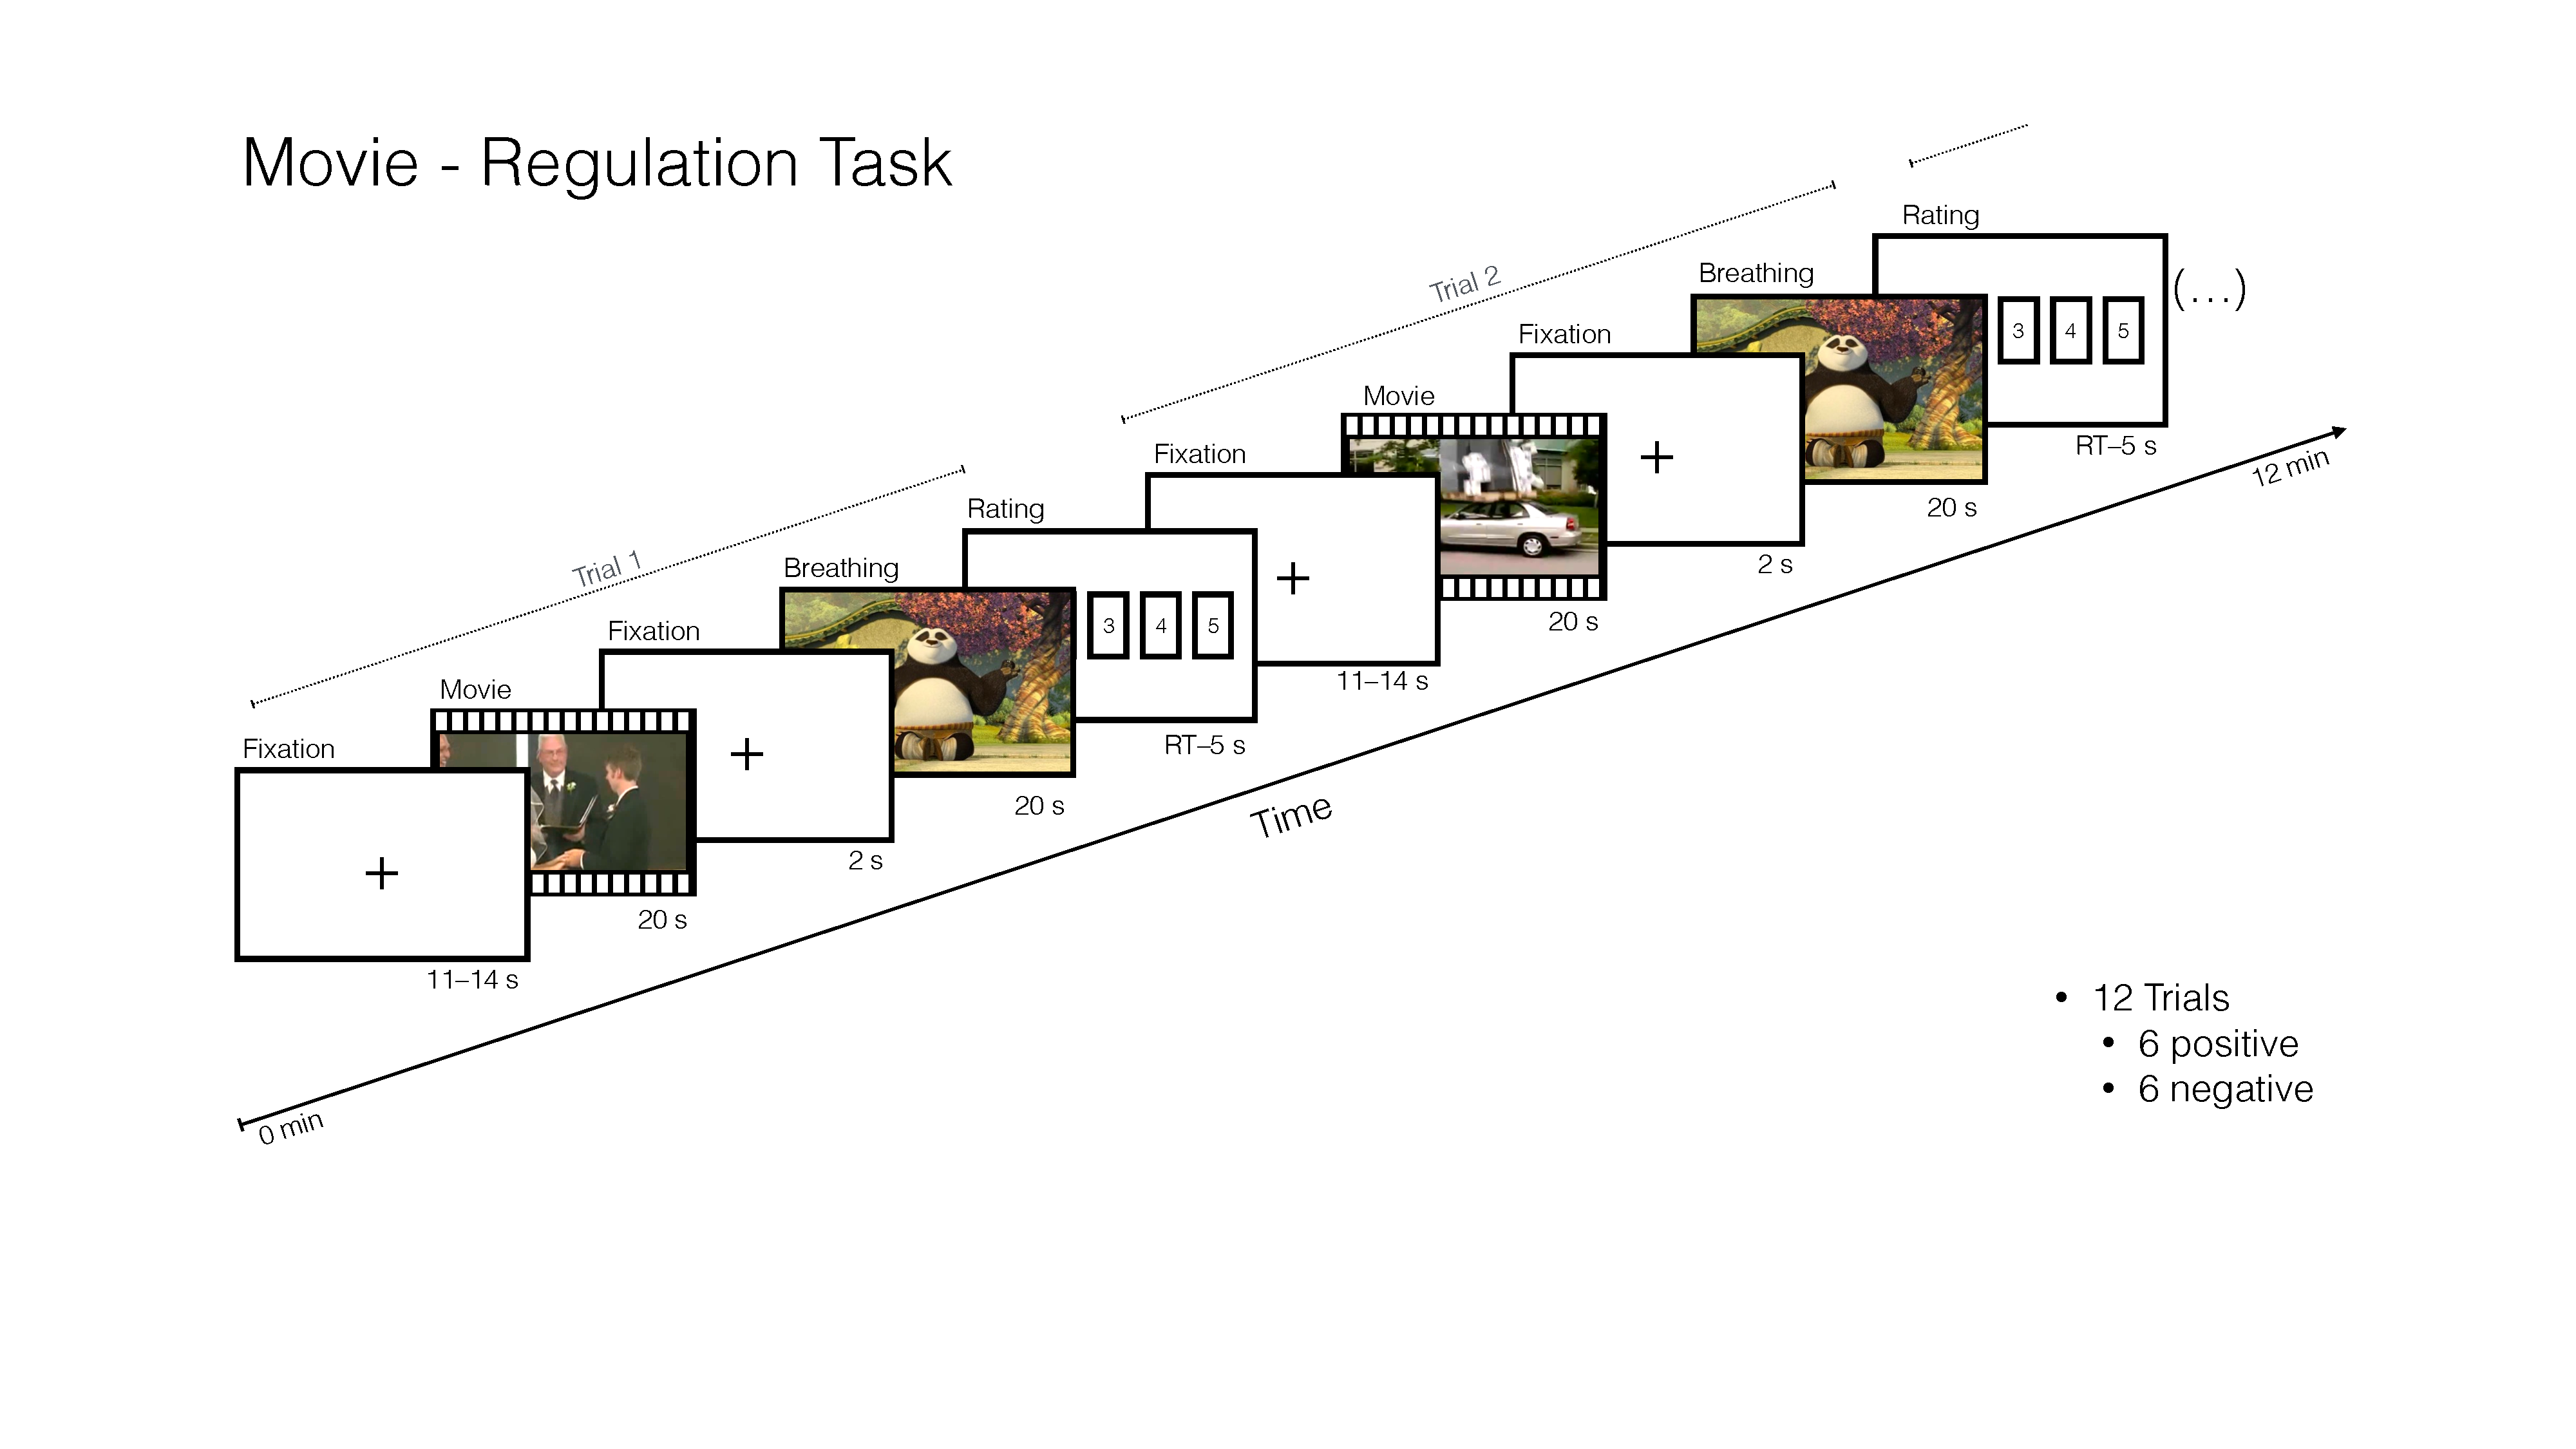
\includegraphics[width=1\textwidth]{images/Ch5/Ch5_movieRegTask.pdf}
\vspace*{5mm}
\caption{\textbf{The movie-regulation task paradigm. } After instructions are shown on the screen and read out loud, the first trial starts with a fixation cross of variable duration, followed by a 20 s-long video. At the end of the video presentation, participants must rate it on a scale from 1 to 5, where 1 represents "negative" and 5 indicates "positive". This is followed by a 30 s interval where participants are asked to concentrate on their breathing. Each trial lasts roughly one minute, and the total protocol includes 12 such trials.  }
\label{fig:videoReg_task} 
\end{figure*}










\subsubsection{MRI acquisition} 
MRI data were acquired on a Siemens 3T Magnetom Prisma scanner at Campus Biotech, Geneva, Switzerland. Structural T1-weighted MP-RAGE (Magnetization Prepared Rapid Gradient Echo) sequences were acquired using the following parameters: voxel size = 0.9 x 0.9 x 0.9 mm; repetition time (TR)~=~2300 ms; echo time (TE) = 2.32 ms; inversion time (TI) = 900 ms; flip angle (FA)~=~8°; field of view (Fov) = 240 mm. Functional images were T2*-weighted with a multislice gradient-echo-planar imaging (EPI) sequence of 64 slices; voxel size = 2 x 2 x 2 mm; TR = 720 ms; TE = 33 ms; Fov = 208 mm. In addition, a fieldmap was acquired every time a participant entered the scanner, with TR = 627 ms; TE1 = 5.19 ms; TE2 = 7.65 ms; and FA = 60°.

\subsubsection{MRI data preprocessing} 
All data were preprocessed using SPM12 (Wellcome Department of Imaging Neuroscience, UCL, UK) in MATLAB R2019a (The MathWorks, Inc., Natick, Massachusetts, United States). The fMRI images from each participant were spatially realigned and unwarped, respectively, to correct for motion artefacts and potential geometric distortions. The unwarping step brings two main advantages: it improves the co-registration between structural and functional images, and reduces the distortion variability across subjects during spatial normalization to a common space \citep{Hutton2002}. Functional images were then coregistered to structural images in subject space and smoothed with a Gaussian filter of full width at half maximum (FWHM) = 6 mm. 

In order to approximate BOLD signals as much as possible to actual brain data, one of the initial steps in PPI-CAPs analysis is to deconvolve the time series with the haemodynamic response function \citep{Freitas2020}. To this end, here we apply total activation (TA) deconvolution \citep{Karahanoglu2013}, a method based on sparse spatio-temporal priors to uncover the underlying activity-inducing signal of fMRI without relying on timing information.

After Total Activation deconvolution, data were warped into MNI (Montreal Neurologic Institute) space via a study-specific DARTEL (Diffeomorphic Anatomical Registration Through Exponentiated Lie algebra) template to be allow group level comparisons. This normalisation method has been shown to be robust to age differences in participants from the age of 7 \citep{ASHBURNER1998, Burgund2002} and is among the top ranked currently available deformation algorithms \citep{Klein2009}.  


\subsubsection{Head motion} 
Head motion was assessed in terms of framewise displacement (FD; \citeauthor{Power2014a}, \citeyear{Power2014a}). Two TB and fourteen PTB subjects for whom more than 20\% of frames would be affected by motion (that is, frames with FD > 0.5 mm, one frame before, and two after those) were excluded from further analyses. For the remaining subjects, total head motion was quite low in both groups: In the control group, for the first fMRI run the mean FD per frame was 0.159 mm with a standard deviation (SD) of $\pm$ 0.05 mm; for the second run the mean FD was 0.154 mm $\pm$ 0.05 mm; In the Preterm group, for the first fMRI run the mean FD per frame was 0.163 mm with a standard deviation (SD) of $\pm$ 0.05 mm; for the second run the mean FD was 0.165 mm $\pm$ 0.06 mm. The two groups did not significantly differ in mean FD (unpaired t-test, p = 0.65). % \add{check if excluded preterms had significantly more cognitive difficulties than remaining ones}

\subsubsection{fMRI analysis} 
To explore moment-to-moment changes in functional connectivity during movie watching or breathing intervals and to see how this changes across groups, we employed a psychophysiological interaction of co-activation patterns (PPI-CAPs) analysis \citep{Freitas2020}. This approach selects moments in which a seed is highly active and clusters frames based on their activation patterns, allowing positive and negative polarities of the same pattern (that is, moments in which activation patterns have completely opposite signs) to be grouped together. It is then possible to test, for each obtained PPI-CAP, whether it varies according to the seed activity, the task progression, or an interaction between the two. 

For this study we selected the dorsal anterior cingulate cortex (ACC) as a seed, as it is a key node of the Salience Network and has been previously shown to be affected by preterm birth in studies involving both static \citep{White2014,Daamen2015,Lordier2019} and dynamic (Chapter \ref{chapter:ch3}) analyses. As all of these studies involved resting-state paradigms so, to the best of our knowledge, this is the first investigation of task-related dynamic ACC connectivity in this population. In addition, to show that interesting task-related dynamics may be found independently of the seed choice, we also conducted the analysis using the PCC as a seed given its description as a hub region \citep{Andrews-hanna2010}, and its wide variety of connection arrangements \citep{Lin2017}, including during internally- \citep{Raichle2001} and externally-oriented cognition  \citep{Freitas2020}. These additional results can be found in Supplementary Material Section \ref{sm_pcc_ppicaps}. In both cases, 30\% of the frames in which the seed was most highly (de)active were selected as a trade-off between using less data while keeping enough frames to obtain stable results \citep{Freitas2020}. The clustering step was performed across both groups together, to avoid the problem of matching similar PPI-CAPs between groups if these were calculated separately. 

To identify the optimal number of PPI-CAPs that must be retrieve, we performed a Consensus Clustering analysis\citep{Monti2003}. This approach applies K-means clustering on several subsamples of the data and calculates the \textit{consensus matrix} $\mathcal{M}$. Each element $\mathcal{M}(a,b)$ indicates the fraction of subsamples in which two frames $a$ and $b$ were both retained in the subsample and clustered together. The optimal number of clusters can then be inferred by visual inspection of the ordered matrix $\mathcal{M}$, as well as of the cumulative distribution function (CDF) of $\mathcal{M}$  for different values of $k$. Once the final k was identified, the final clustering step was performed using 100 replicates. 


\subsubsection{Network assignment}
After PPI-CAPs were obtained in the clustering step, we identified the regions and networks highlighted in each pattern by comparing them to those from previous studies using two approaches. First, we compared them to the 7 functional networks identified by \cite{Yeo2011}. This was achieved by calculating what proportion of each functional network was activated or deactivated in each PPI-CAP, and then applying the Hungarian Algorithm \cite{Munkres1957} to the resulting matrix, to assign networks to each pattern.  In addition, we uploaded the PPI-CAPs' files to NeuroSynth.org \citep{Wager2011a} and investigated the regions most associated with each PPI-CAP according with the automated meta-analysis tool. 


\subsubsection{Significance assessment}
For each PPI-CAP, we tested 3 main (Seed; Task; Group) and 3 interaction (Seed vs. Task, or PPI; Group vs. Task; and Group vs. Seed).
If a PPI-CAP has a strong main or interaction effect, the polarity of the frames that constitute it will tend to correlate with the sign of that effect for the same time points. To visualise if this is the case, we can thus generate confusion matrices for each effect and PPI-CAP. When there is a strong correlation, the higher values of a confusion matrix will tend to load on one of its diagonals, and the relevance of this relationship can be measured by taking the matrix's determinant, or \textit{det-index}. To test whether this value is significant, we generate null distributions by performing random permutations of the effect of interest's labels and re-calculate the det-index each time. Finally, we see where the real det-index stands in the distribution (Figure~\ref{PPI_CAPs_fw}F).
For this study, we performed 3000 random permutations for each test. We disclose the null distributions and uncorrected p-values in the Supplementary Figures for this chapter and, in the Results Section, indicate  effects with significance level $\alpha$ \textsubscript{$0.05/6$} = 0.008), to correct for the number of PPI-CAPs.


\subsubsection{Investigation of seed heterogeneity}
Finally, we investigated the source of the seed activity to test how heterogeneous the seed was. To this end, we clustered the seed's voxelwise time courses --- signed after z-scoring --- into three subgroups. We then projected these groups back onto the brain to identify possible subdivisions of the seed and to better understand where the averaged signal likely came from. 




\subsection{Results}

\subsubsection{Consensus clustering}
We performed consensus clustering using a K range from 3 to 20 to identify the most stable number of clusters for our data. Visual inspection of the confusion matrices for each value of K, as well as the plot of the proportion of ambiguously clustered frames for each case, identified K~=~6 as a clear optimal value. These results can be found in Supplementary Figure \ref{fig:app_acc_k}

\subsubsection{Six patterns from ACC-based PPI-CAPs}
Clustering ACC-selected frames  yielded the patterns shown in Figure \ref{fig:acc_ppicaps}. According to the Hungarian Algorithm-based assignment of networks each PPI-CAP was identified as the following: PPI-CAP\textsubscript{1} corresponds to an activated somatomotor network (SMN) and deactivated default mode network;  PPI-CAP\textsubscript{2} is assigned to an activated ventral attention Network, also known as salience network (SN),  and deactivated limbic; PPI-CAP\textsubscript{3} contains an activated Visual and deactivated fronto-parietal network (FPN); PPI-CAP\textsubscript{4} includes an activated dorsal attention (DAN) and deactivated visual network; PPI-CAP\textsubscript{5} has an activated FPN and deactivated SMN; and PPI-CAP\textsubscript{6} includes an activated limbic and deactivated DAN. As visual inspection of Figure \ref{fig:acc_ppicaps} suggests, some CAPs had similarities with more than one network. The full similarity matrix can be found in Figure \ref{fig:app_acc_munkres} in the Supplementary Material for this chapter. For simplicity, we will interpret the results based on the assigned networks.









\begin{figure*}[h!]
\centering
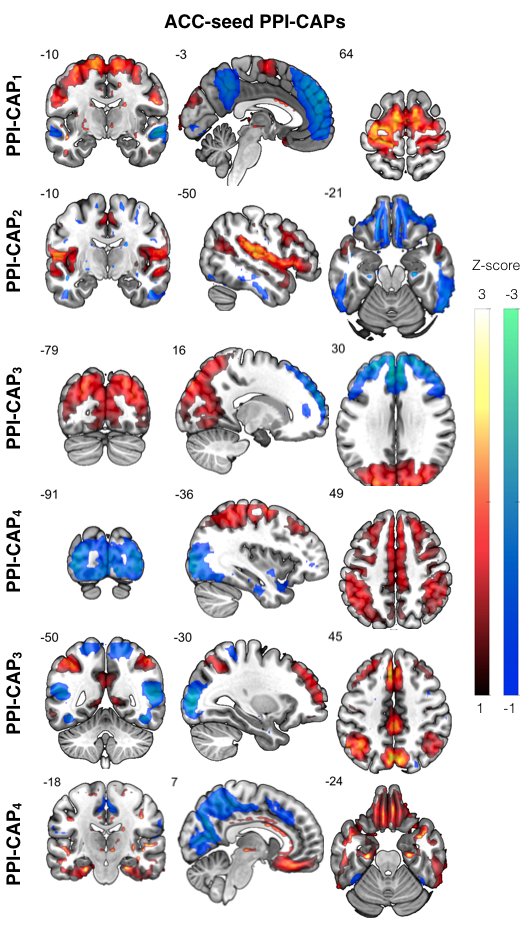
\includegraphics[width=0.75\textwidth]{images/Ch5/Ch5_ACC_PPI-CAPs.png}
\caption{\textbf{PPI-CAPs focused on the ACC yield six dynamic patterns.} Using K~=~6 for the clustering step as defined in Figure \ref{fig:app_acc_k} yielded the six PPI-CAPs above. Each row corresponds to one PPI-CAP, numbers indicate slice coordinates in MNI space.}
\label{fig:acc_ppicaps}
\end{figure*}



\subsubsection{Main and interaction effects}
For each PPI-CAP, we tested for main and interaction effects by checking if the flipping of each pattern correlates with the sign of each effect. The resulting confusion matrices can be seen in Figure \ref{fig:acc_cm}. Each row corresponds to a PPI-CAP. Permutation testing then identified which of these effects were significant, which can be seen in Figure \ref{fig:app_acc_stats} in the Supplementary Material.



\begin{figure*}[h!]
\centering
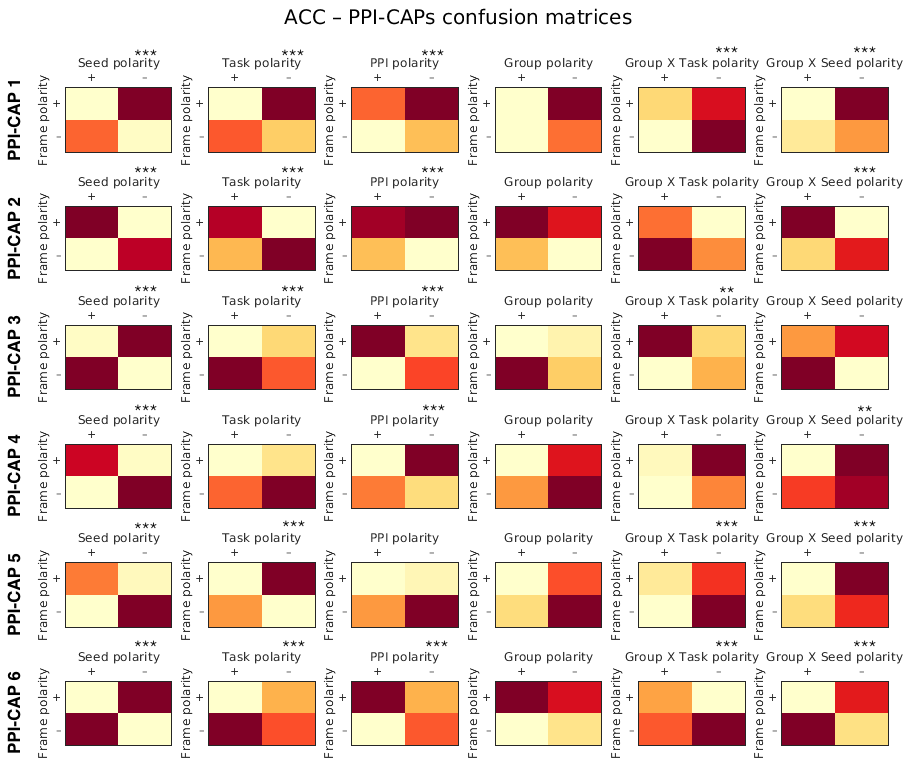
\includegraphics[width=1\textwidth]{images/Ch5/Ch5_ACC_cm.png}
\caption{\textbf{ACC-seed PPI-CAPs show a variety of main and interaction effects.} To identify main and interaction effects for each PPI-CAP, confusion matrices show how often the sign of a PPI-CAP switches in the same way as each of the effects. We tested three main effects (Seed; Task; and Group) and three interaction effects (Seed vs. Task (PPI); Group vs. Seed; and Group vs. Task). The signs for each effect are as follows: Seed --- positive and negative signs correspond to frames when the seed was activated of deactivated, respectively;  Task --- positive signs correspond to "Movie Watching" while negative signs correspond to moments of "Emotion Regulation"; Group --- positive signs correspond to fullterm controls, while negative signs correspond to preterm-born individuals. Interaction signs are calculated as element-by-element multiplication of the main effect signs. Light yellow indicates the lowest number of frames, while dark red indicates the highest number of frames. ***~=~p<0.001; **~=~P<0.008. Significance level $\alpha$ \textsubscript{$0.05/6$} = 0.008).}
\label{fig:acc_cm}
\end{figure*}


\paragraph{Main effects:}
All the PPI-CAPs showed a significant seed effect at $p~<~0.001$ (Figure \ref{fig:app_acc_stats}, first column). As the direction of the diagonals in the first column of Figure \ref{fig:acc_cm} suggest, PPI-CAPs 2, 4 and 5 we positively correlated with the seed, while PPI-CAPs 1, 3 and 6 were negatively correlated with it. PPI-CAP 2 was positively correlated with the task ($p~<~0.001$), meaning that the salience network was more active during the Movie Watching Task. In contrast, PPI-CAPs 1, 3, 5 and 6 were anti-correlated with the task, meaning that the areas shown in red for these patterns in Figure \ref{fig:acc_ppicaps} tended to be more active during the Emotion Regulation task (all, $p~<~0.001$). Only PPI-CAP 1 showed a group effect, occurring more often in the preterm group ( $p~<~0.03$, uncorrected), with a tendency to appear more often in its positive configuration.

\paragraph{Interaction effects:}
PPI-CAPs 1, 3, and 6 show  a positive interaction between seed and task (PPI effect), meaning that these patterns correlate with the seed more during Movie Watching and are anti-correlated with the ACC during  Emotion Regulation (all, $p~<~0.001$). In contrast, PPI-CAPs 2 and 4 show a negative PPI effect, such that they correlate more with the seed during Emotion Regulation (all, $p~<~0.001$). PPI-CAPs 1 ($p~<~0.001$), 3 ($p~=~0.002$), 5 ($p~<~0.001$) and 6 ($p~<~0.001$) have a positive group versus task interaction, such that during Movie Watching, the regions shown in red for these patterns are more often activated in controls than in preterms, while during Emotion Regulation these regions are also more often de-activated for this group. Finally, PPI-CAP 2 has a positive group versus seed interaction effect ($p~<~0.001$), while PPI-CAPs 1 ($p~<~0.001$), 4 ($p~=~0.003$), 5 ($p~<~0.001$), and 6 ($p~<~0.001$) have a negative group versus seed interaction effect.


\subsubsection{Seed heterogeneity}
Clustering the seed's voxels' based on their signed time courses revealed three clear spatial subdivisions. The averaged seed activation seems to come mainly from subdivisions one and two, with subdivision three having a temporal pattern that resembled the former less. Figure \ref{fig:acc_subdivisions} illustrates this result. 


\begin{figure*}[h!]
\centering
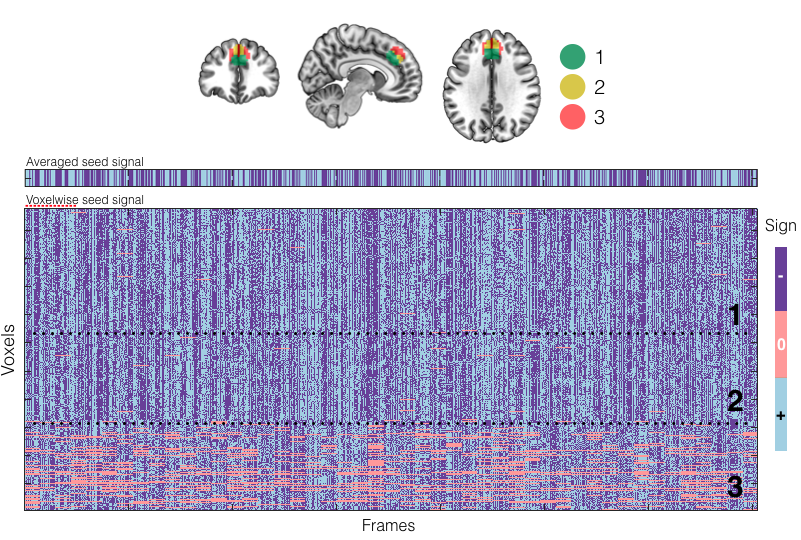
\includegraphics[width=1\textwidth]{images/Ch5/Ch5_ACC_subdivisions.png}
\caption{\textbf{ACC-seed subdivisions based on temporal activity.} Temporally clustering the voxelwise seed activity's sign (large rectangle) across all subjects yielded three spatial subdivisions of the dorsal anterior cingulate cortex, indicated in green, yellow and red in the brain plot. The activity of voxels within regions one and  two (as indicated by the top two layers of the large rectangle) resembled more closely and thus seem to be driving the seed's averaged signal (top rectangle). }
\label{fig:acc_subdivisions}
\end{figure*}



\subsection{Discussion}
In this study we investigated dynamic functional connectivity in the context of a task involving movie watching and emotional regulation in a preterm-born population of young adolescents. We employed a state-of-the-art method to uncover several patterns of co-activation with an anterior cingulate cortex (ACC) seed and analyse their relationship with three main effects (namely seed; task; and group), as well as three interaction effects (namely seed versus task; group versus task; and group versus seed). We identified several patterns with a significant effect, many of which involved differences across the two groups, revealing dynamic aspects of brain function in the preterm population that had not been uncovered before. 

Our exploration of ACC-based connectivity patterns revealed several reproducible PPI-CAPs, with six being the optimal number of repeatable patterns. Previous studies had shown a wide variety of possible brain states in connection with other brain regions such as the posterior cingulate cortex \citep{Liu2013a,Lin2017,Freitas2020}. The ACC, in turn, has often come up in BOLD variability studies, including some involving clinical populations \citep{Zoller2017,Zhang2020}, suggesting this brain region's high flexibility and that dynamic aspects of its function and connectivity may be implicated in the neurological mechanisms of clinical disorders. While Chapter \ref{chapter:ch3} investigated o the best of our knowledge this is the first study to  have explored the task-related dynamic connectivity range of the ACC.


Only one PPI-CAP had a pure group effect close to significance. This was PPI-CAP 1, with somatomotor (SMN) areas being more highly active, while the default mode network (DMN) was deactive, in preterm-born children throughout the experiment. In addition, the group versus polarity effect indicates that it appears more often when this group is performing the movie watching task (note the darker colours on the right side of the corresponding confusion matrix in Figure \ref{fig:acc_cm}). In typically developing individuals, motor stimulation is related to contralateral activation of the motor cortex. Furthermore, not only physical stimulation, but even just the act of watching someone else move, or of imagining oneself moving, already generates similar activation \citep{Butler2006}. Studies involving somatomotor stimulation in preterm-born infants, however, have often found bilateral (as opposed to only contralateral) activation of the motor cortex in response to unilateral stimulation \citep{Heep2009a,Arichi2010,Allievi2016}. Many of the the videos shown during Movie Watching blocks involve high movement such as sports scenes of families playing football. Taken together, the above facts may justify not only the occasional appearance of motor-related areas during this experiment, but also why it appears more for the preterm group. Further analyses based on transients \citep{Karahanoglu2015a,Freitas2020} would help to disentangle the spatiotemporal overlapping of the different regions included in the PPI-CAP in this case.

Interestingly, PPI-CAP 6, which includes the limbic network (LN) and the dorsal attention network (DAN) with opposite signs, shows both a group versus task and a group versus seed interaction effects. In controls, the LN is more often active when movie watching than during emotional regulation, while the opposite is true for the preterm group. It is also more deactivated (and the DAN activated) when the preterm are movie watching. These results are in line with previous results which found altered structural connectivity of the cortico-basal-thalamo-cortical loop and the limbic system, which are essential for socio-emotional processing \citep{Olson2007,Braun2011}, in preterm-born school age children as compared to term-born controls \citep{Fischi-Gomez2015,Fischi-Gomez2016a}.

The investigation of seed homogeneity by clustering voxels based on their temporal features revealed three spatial subdivisions. This was done in a data-driven way, showing that there is a high level of consistency between neighbouring voxels. It also highlights that the seed itself is not entirely homogeneous and that the effects we found mainly related to the ventral part of the dorsal anterior cingulate cortex. 

Taken  together, the results presented here underline the potential of dynamic analyses to uncover brain function relationships that cannot be examined using traditional static methodologies. The potential to study these dynamic features in combination with behavioural and clinical outcomes proves a compelling direction for future research. 






\subsection*{Considerations and future avenues}

Although we identifies a variety of patterns that co-activate with the ACC, it is not possible to know whether all the brain regions contained in each pattern activated (or deactivated) simultaneously --- and it probably is not the case. Future studies would benefit from combining the PPI-CAPs approach with a method that extracts \textit{transients}, or moments of change, from the data, and only then performs the clustering step \citep{Karahanoglu2015a,Freitas2020}. This would help clarify the co-occurrence of certain networks with opposite signs in some of the PPI-CAPs we uncovered. 

This study includes a task block where participants are asked to focus on their breathing. The very act of concentration one one's breathing has been shown to alter breathing patterns \citep{Conrad2007}, which may cause changes not only in motion, but also CO\textsubscript{2} levels \citep{Western1988}. A recent study by \citet{Chen2020} has shown that increased CO\textsubscript{2} levels induce vasodilation and an increase in blood flow, which may drive so-called "physiological networks". Thus, including physiological measures in a subsequent analysis would help control for these potential confounds when exploring task effects.


Another compelling next step would be to explore potential relationships between the occurrence of patterns identified here with behavioural and clinical measures from the participants. For example, does the occurrence of PPI-CAP 6, which has a strong emotional component, correlate with scores of emotional aptitude in these young adolescents? Future studies will help clarify this point.

Finally, recent studies have looked into another aspect of brain dynamics called quasi-periodic patterns (QPP)\citep{Majeed2011}. This approach assumes that brain activity and BOLD fluctuations are dominated by a slow propagation of activity involving the DMN task positive networks \citep{Abbas2019}. The QPPs can then be tested on their spatiotemporal pattern, frequency and strength, which is useful to identify whether not only the existence of different patterns of activity \textit{per se}, but also \textit{e.g.} the specific order in which they appear, brings novel information about clinical populations \citep{Briend2020}.


% Salience shows more during Movie Watching, makes sense as there's much more stimulation. 
